\documentclass{beamer}

% xcolor and define colors -------------------------
\usepackage{xcolor}

% https://www.viget.com/articles/color-contrast/
\definecolor{purple}{HTML}{5601A4}
\definecolor{navy}{HTML}{0D3D56}
\definecolor{ruby}{HTML}{9a2515}
\definecolor{alice}{HTML}{107895}
\definecolor{daisy}{HTML}{EBC944}
\definecolor{coral}{HTML}{F26D21}
\definecolor{kelly}{HTML}{829356}
\definecolor{cranberry}{HTML}{E64173}
\definecolor{jet}{HTML}{131516}
\definecolor{asher}{HTML}{555F61}
\definecolor{slate}{HTML}{314F4F}

% Mixtape Sessions
\definecolor{picton-blue}{HTML}{00b7ff}
\definecolor{violet-red}{HTML}{ff3881}
\definecolor{sun}{HTML}{ffaf18}
\definecolor{electric-violet}{HTML}{871EFF}

% Main theme colors
\definecolor{accent}{HTML}{00b7ff}
\definecolor{accent2}{HTML}{871EFF}
\definecolor{gray100}{HTML}{f3f4f6}
\definecolor{gray800}{HTML}{1F292D}


% Beamer Options -------------------------------------

% Background
\setbeamercolor{background canvas}{bg = white}

% Change text margins
\setbeamersize{text margin left = 15pt, text margin right = 15pt} 

% \alert
\setbeamercolor{alerted text}{fg = accent2}

% Frame title
\setbeamercolor{frametitle}{bg = white, fg = jet}
\setbeamercolor{framesubtitle}{bg = white, fg = accent}
\setbeamerfont{framesubtitle}{size = \small, shape = \itshape}

% Block
\setbeamercolor{block title}{fg = white, bg = accent2}
\setbeamercolor{block body}{fg = gray800, bg = gray100}

% Title page
\setbeamercolor{title}{fg = gray800}
\setbeamercolor{subtitle}{fg = accent}

%% Custom \maketitle and \titlepage
\setbeamertemplate{title page}
{
    %\begin{centering}
        \vspace{20mm}
        {\Large \usebeamerfont{title}\usebeamercolor[fg]{title}\inserttitle}\\
        {\large \itshape \usebeamerfont{subtitle}\usebeamercolor[fg]{subtitle}\insertsubtitle}\\ \vspace{10mm}
        {\insertauthor}\\
        {\color{asher}\small{\insertdate}}\\
    %\end{centering}
}

% Table of Contents
\setbeamercolor{section in toc}{fg = accent!70!jet}
\setbeamercolor{subsection in toc}{fg = jet}

% Button 
\setbeamercolor{button}{bg = accent}

% Remove navigation symbols
\setbeamertemplate{navigation symbols}{}

% Table and Figure captions
\setbeamercolor{caption}{fg=jet!70!white}
\setbeamercolor{caption name}{fg=jet}
\setbeamerfont{caption name}{shape = \itshape}

% Bullet points

%% Fix left-margins
\settowidth{\leftmargini}{\usebeamertemplate{itemize item}}
\addtolength{\leftmargini}{\labelsep}

%% enumerate item color
\setbeamercolor{enumerate item}{fg = accent}
\setbeamerfont{enumerate item}{size = \small}
\setbeamertemplate{enumerate item}{\insertenumlabel.}

%% itemize
\setbeamercolor{itemize item}{fg = accent!70!white}
\setbeamerfont{itemize item}{size = \small}
\setbeamertemplate{itemize item}[circle]

%% right arrow for subitems
\setbeamercolor{itemize subitem}{fg = accent!60!white}
\setbeamerfont{itemize subitem}{size = \small}
\setbeamertemplate{itemize subitem}{$\rightarrow$}

\setbeamertemplate{itemize subsubitem}[square]
\setbeamercolor{itemize subsubitem}{fg = jet}
\setbeamerfont{itemize subsubitem}{size = \small}

% Special characters

\usepackage{collectbox}

\makeatletter
\newcommand{\mybox}{%
    \collectbox{%
        \setlength{\fboxsep}{1pt}%
        \fbox{\BOXCONTENT}%
    }%
}
\makeatother






% Links ----------------------------------------------

\usepackage{hyperref}
\hypersetup{
  colorlinks = true,
  linkcolor = accent2,
  filecolor = accent2,
  urlcolor = accent2,
  citecolor = accent2,
}


% Line spacing --------------------------------------
\usepackage{setspace}
\setstretch{1.2}


% \begin{columns} -----------------------------------
\usepackage{multicol}


% Fonts ---------------------------------------------
% Beamer Option to use custom fonts
\usefonttheme{professionalfonts}

% \usepackage[utopia, smallerops, varg]{newtxmath}
% \usepackage{utopia}
\usepackage[sfdefault,light]{roboto}

% Small adjustments to text kerning
\usepackage{microtype}



% Remove annoying over-full box warnings -----------
\vfuzz2pt 
\hfuzz2pt


% Table of Contents with Sections
\setbeamerfont{myTOC}{series=\bfseries, size=\Large}
\AtBeginSection[]{
        \frame{
            \frametitle{Roadmap}
            \tableofcontents[current]   
        }
    }


% Tables -------------------------------------------
% Tables too big
% \begin{adjustbox}{width = 1.2\textwidth, center}
\usepackage{adjustbox}
\usepackage{array}
\usepackage{threeparttable, booktabs, adjustbox}
    
% Fix \input with tables
% \input fails when \\ is at end of external .tex file
\makeatletter
\let\input\@@input
\makeatother

% Tables too narrow
% \begin{tabularx}{\linewidth}{cols}
% col-types: X - center, L - left, R -right
% Relative scale: >{\hsize=.8\hsize}X/L/R
\usepackage{tabularx}
\newcolumntype{L}{>{\raggedright\arraybackslash}X}
\newcolumntype{R}{>{\raggedleft\arraybackslash}X}
\newcolumntype{C}{>{\centering\arraybackslash}X}

% Figures

% \imageframe{img_name} -----------------------------
% from https://github.com/mattjetwell/cousteau
\newcommand{\imageframe}[1]{%
    \begin{frame}[plain]
        \begin{tikzpicture}[remember picture, overlay]
            \node[at = (current page.center), xshift = 0cm] (cover) {%
                \includegraphics[keepaspectratio, width=\paperwidth, height=\paperheight]{#1}
            };
        \end{tikzpicture}
    \end{frame}%
}

% subfigures
\usepackage{subfigure}


% Highlight slide -----------------------------------
% \begin{transitionframe} Text \end{transitionframe}
% from paulgp's beamer tips
\newenvironment{transitionframe}{
    \setbeamercolor{background canvas}{bg=accent!40!black}
    \begin{frame}\color{accent!10!white}\LARGE\centering
}{
    \end{frame}
}


% Table Highlighting --------------------------------
% Create top-left and bottom-right markets in tabular cells with a unique matching id and these commands will outline those cells
\usepackage[beamer,customcolors]{hf-tikz}
\usetikzlibrary{calc}
\usetikzlibrary{fit,shapes.misc}

% To set the hypothesis highlighting boxes red.
\newcommand\marktopleft[1]{%
    \tikz[overlay,remember picture] 
        \node (marker-#1-a) at (0,1.5ex) {};%
}
\newcommand\markbottomright[1]{%
    \tikz[overlay,remember picture] 
        \node (marker-#1-b) at (0,0) {};%
    \tikz[accent!80!jet, ultra thick, overlay, remember picture, inner sep=4pt]
        \node[draw, rectangle, fit=(marker-#1-a.center) (marker-#1-b.center)] {};%
}

\usepackage{breqn} % Breaks lines

\usepackage{amsmath}
\usepackage{mathtools}

\usepackage{pdfpages} % \includepdf

\usepackage{listings} % R code
\usepackage{verbatim} % verbatim

% Video stuff
\usepackage{media9}

% packages for bibs and cites
\usepackage{natbib}
\usepackage{har2nat}
\newcommand{\possessivecite}[1]{\citeauthor{#1}'s \citeyearpar{#1}}
\usepackage{breakcites}
\usepackage{alltt}

% tikz
\usepackage{tikz}
\usepackage{pgfplots}
\usetikzlibrary{calc, positioning, decorations.pathreplacing, arrows.meta, intersections}
\pgfdeclarelayer{bg}
\pgfdeclarelayer{back}
\pgfdeclarelayer{fg}
\pgfsetlayers{bg,main,fg,back}
\usetikzlibrary{shapes,arrows}

% Setup math operators
\DeclareMathOperator{\E}{E} \DeclareMathOperator{\tr}{tr} \DeclareMathOperator{\se}{se} \DeclareMathOperator{\I}{I} \DeclareMathOperator{\sign}{sign} \DeclareMathOperator{\supp}{supp} \DeclareMathOperator{\plim}{plim}
\DeclareMathOperator*{\dlim}{\mathnormal{d}\mkern2mu-lim}
\newcommand\independent{\protect\mathpalette{\protect\independenT}{\perp}}
   \def\independenT#1#2{\mathrel{\rlap{$#1#2$}\mkern2mu{#1#2}}}
\newcommand*\colvec[1]{\begin{pmatrix}#1\end{pmatrix}}

\newcommand{\myurlshort}[2]{\href{#1}{\textcolor{gray}{\textsf{#2}}}}


\begin{document}

\imageframe{./lecture_includes/torino_ai}


% ---- Content ----



\section{Overview}

\begin{frame}{Introduction!}

  \begin{itemize}
	\item I'm Scott Cunningham, Ben H. Williams professor of economics at Baylor University, author of \underline{Causal Inference: the Mixtape}
	\item I work on a variety of eclectic topics including sex work, methamphetamine drug policy, abortion policy, and more recently, detecting and treating self harm in prisons and mails
  \end{itemize}

\end{frame}


\begin{frame}{What is my teaching like}
    \begin{itemize}
        \item I focus on intuition, mechanics, calculations, meaning, assumptions, and coding.
        \item I advocate for data visualization – blending the art and science of causal inference.
        \item I teach with passion, enthusiasm, and deep joy.
        \item I'm not an econometrician, so I sometimes take the scenic route to get to the point.
    \end{itemize}
\end{frame}



\begin{frame}{This week}

  \begin{itemize}
    \item This is a week long course on ``selection on observable'' methods in causal inference: 
    	\begin{enumerate}
	\item Unconfoundedness: Matching, Propensity scores, Regression adjustment
	\item Regression discontinuity design
	\end{enumerate}
  \end{itemize}

\end{frame}




\begin{frame}{Class goals}

  \begin{enumerate}
    \item \textbf{Confidence}: You will feel like you have a good understanding of causal inference so that by the end it doesn't feel all that mysterious or intimidating
    \item \textbf{Comprehension}: You will have learned a lot both conceptually and in the specifics, particularly with regards to issues around identification and estimation
    \item \textbf{Competency}: You will have more knowledge of programming syntax in Stata and R (and python!) so that later you can apply this in your own work
  \end{enumerate}

\end{frame}


%\begin{frame}{Causal Inference table of contents}
%  \centering
%  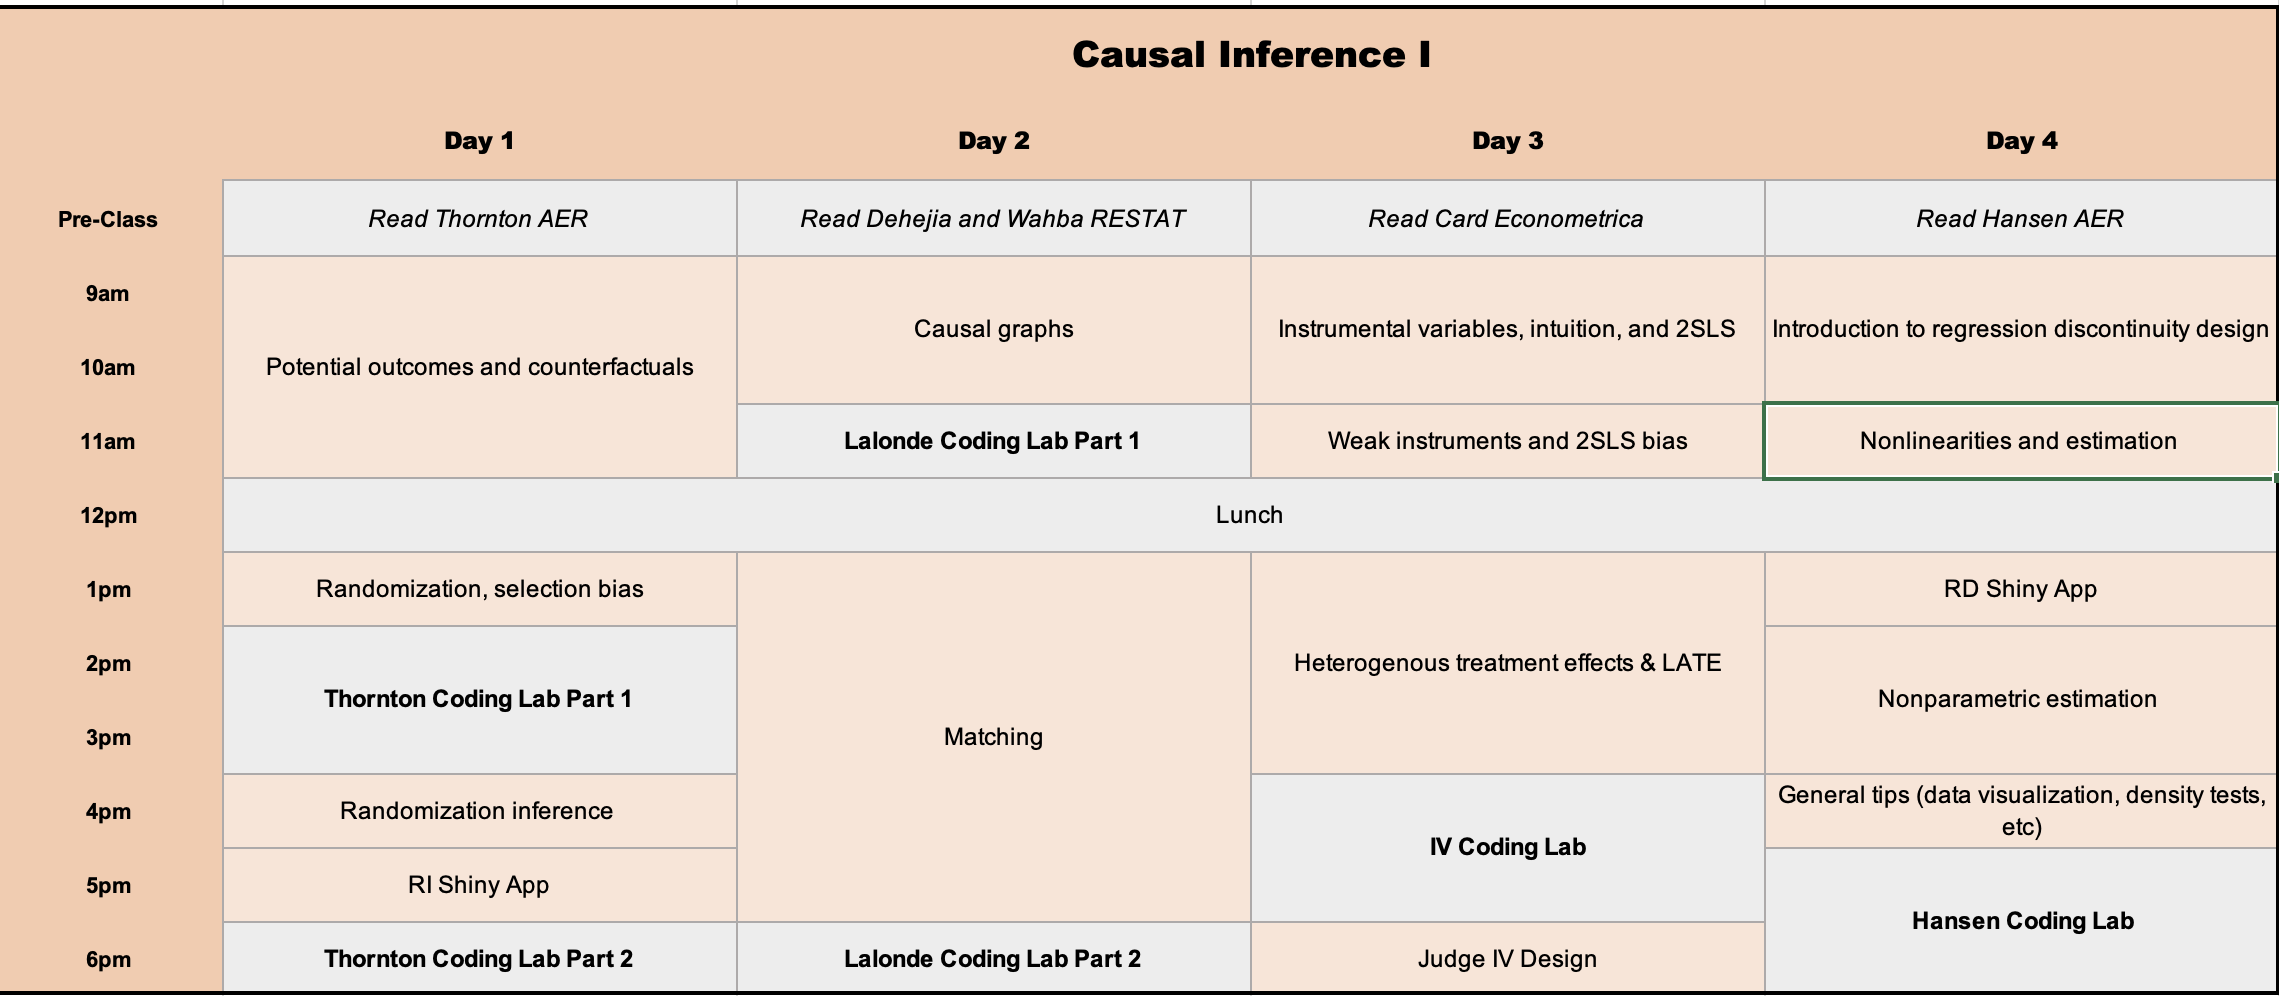
\includegraphics[scale=0.5,height=6.5cm, width=10cm]{./lecture_includes/part1}
%\end{frame}

%\begin{frame}{Causal Inference Part 2}
%  \centering
%  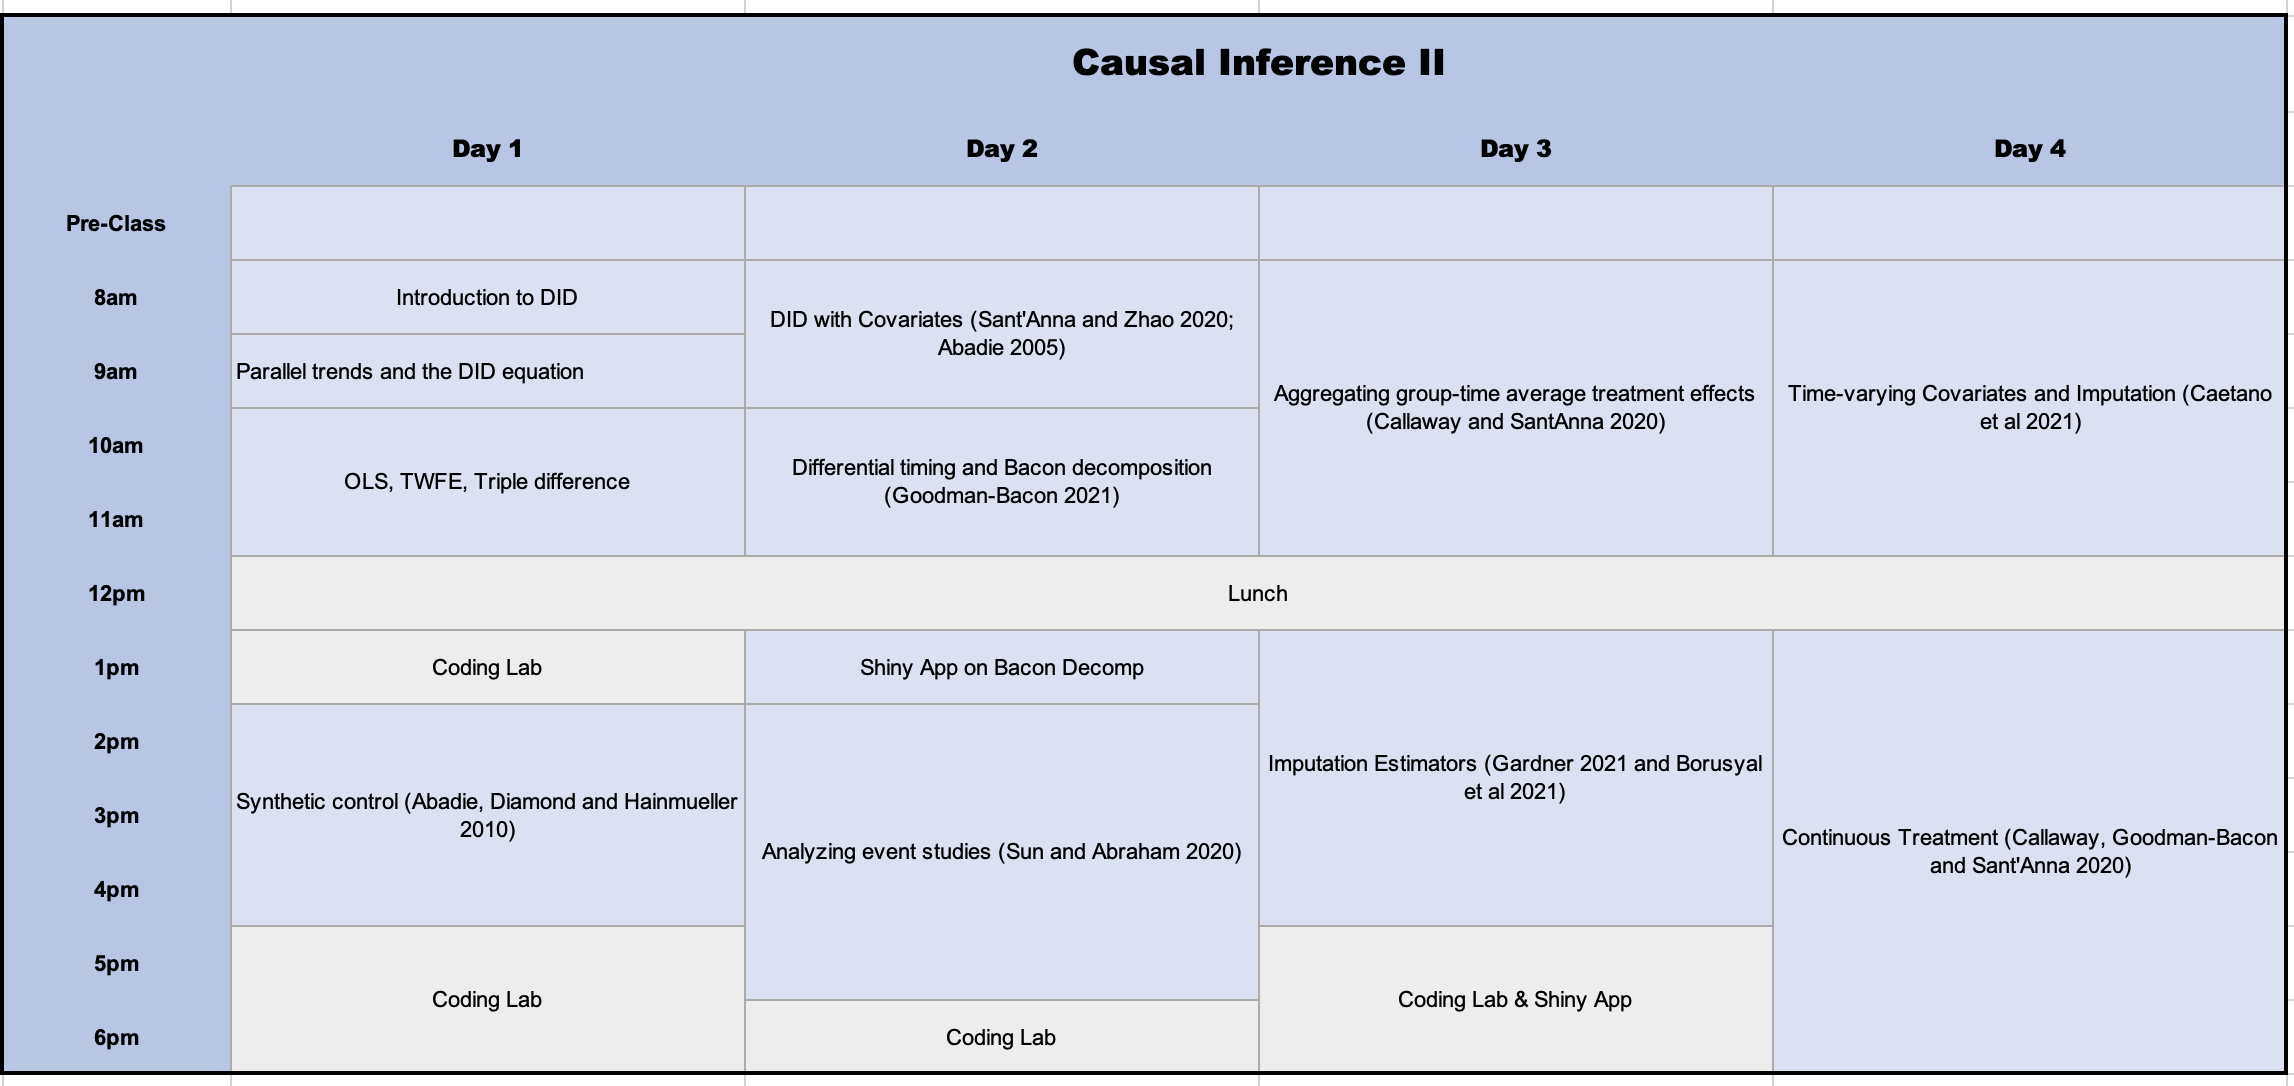
\includegraphics[scale=0.5,height=6.5cm, width=10cm]{./lecture_includes/part2}
%  \url{https://www.mixtapesessions.io/session/ci_II_aug20}
%\end{frame}




\begin{frame}{Class items}

  \begin{itemize}
    \item I'd like for you to listen to three podcast interviews I did this week and write a summary of a paper that I will assign going with each person
    	\begin{enumerate}
	\item Guido Imbens interview alongside the Kolesar, Hull, and Walters "Labor by Design" article"
	\item David Card interview alongside his Nobel speech
	\item Josh Angrist interview alongside his Mainmonides rule paper with Victor Lavy
	\end{enumerate}
\item I've placed readings I hope you find helpful as well as slides on our githut repo at \url{https://github.com/scunning1975/Torino-2024}
  \end{itemize}

\end{frame}




\section{Causality Fallacies}


\begin{frame}{What is Causality?}

\begin{itemize}
\item Causality is metaphysics (what is?); causal inference is epistemology (what is knowledge?) IOW, what makes a causal belief a ``warranted belief''?
\item Causality and causal inference have common sources (e.g., Aristotle, Hume, Mill, Lewis) but we will focus primarily on the experimental design tradition
\item We use the potential outcomes framework of causal inference to build and discuss methods that estimate unbiased and meaningful \textbf{average} causal parameters as defined by that framework
\end{itemize}

\end{frame}


\begin{frame}{Causal Inference vs Prediction}
  \centering
  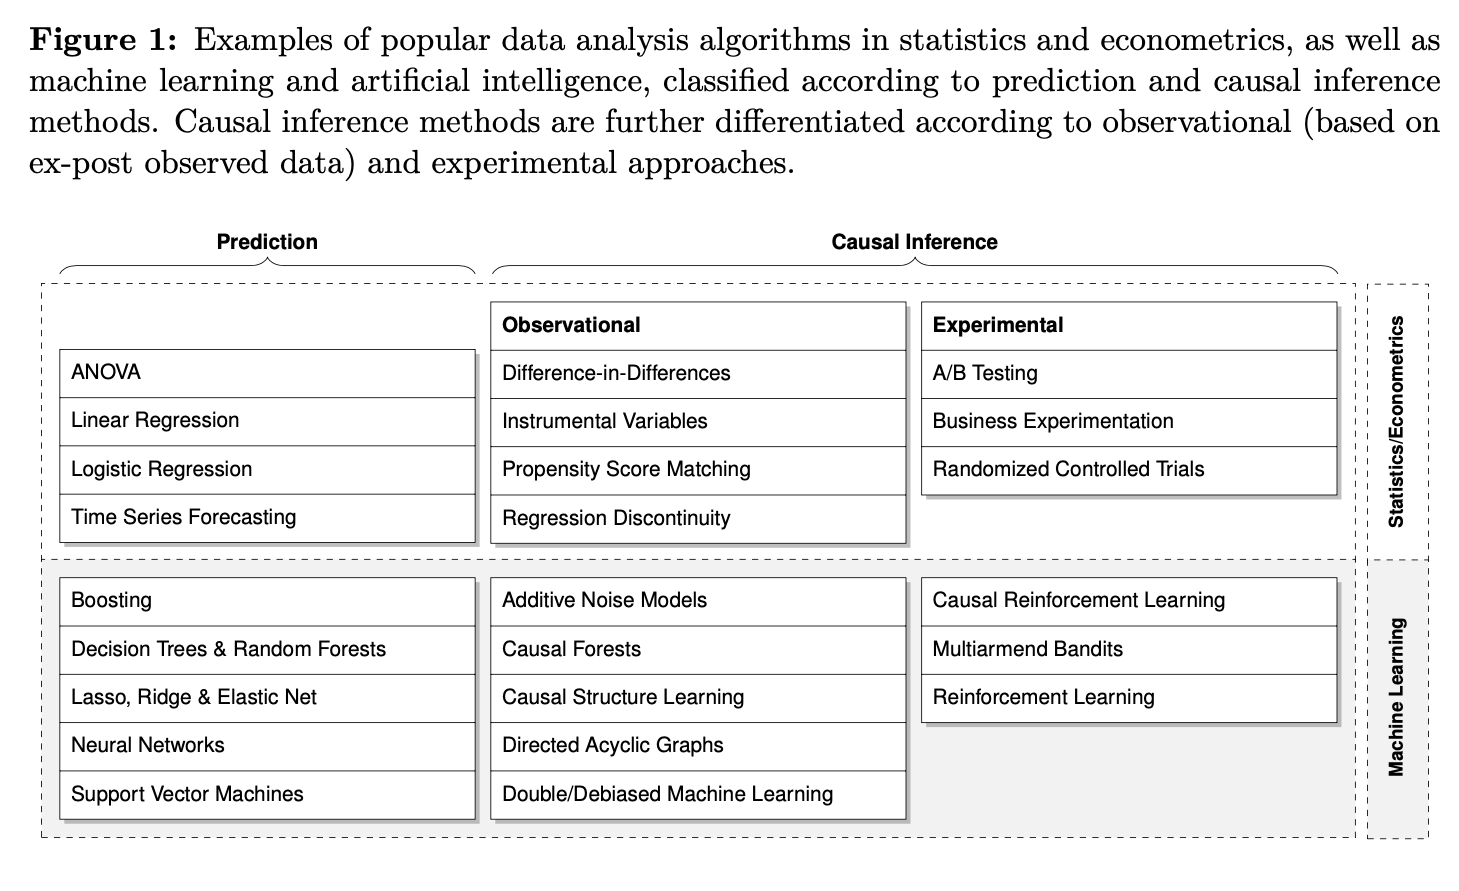
\includegraphics[scale=0.5,height=6.5cm, width=10cm]{./lecture_includes/prediction_causality.png}
\end{frame}

\begin{frame}{Causal Inference vs Prediction}

  \begin{columns}
    \column{0.48\linewidth}
    \centering
    \textbf{Traditional prediction}
    \begin{itemize}
      \item Traditional prediction seeks to detect patterns in data and fit functional relationships between variables with a high degree of accuracy
      \item ``Does this person have heart disease?'', ``How many books will I sell?''
      \item It is not predictions of what effect a choice will have, though
    \end{itemize}
    \column{0.48\linewidth}
    \centering
    \textbf{Causal inference}
    \begin{itemize}
      \item Causal inference is also a type of prediction, but it's a prediction of a \emph{counterfactual} associated with a particular \emph{choice taken}
      \item Causal inference takes that predicted (or imputed) counterfactual and constructs a causal effect that we hope tells us about a future in the event of a similar choice taken
    \end{itemize}
  \end{columns}
\end{frame}



\begin{frame}{Naive causal inference}

  \begin{itemize}
    \item Aliens estimate a model showing a systematic correlation between COVID deaths and ventilators
    \item They conclude doctors are killing patients with ventilators so they come to earth to liberate the patients, but it only makes things worse
    \item Their error was they confused correlation with causality, but deeper than that, they didn't understand how the world worked
    \item \emph{We are the aliens in our research}
  \end{itemize}

\end{frame}

\begin{frame}{\#1: Correlation and causality are different concepts}

  Causal is one unit, correlation is many units
  \begin{itemize}
    \item Causal question: ``If a doctor puts a patient on a ventilator (D), will her covid symptoms (Y) improve?''
    \item Correlation question:  $$\frac{Cov(D,Y)}{\sqrt{Var_D}\sqrt{{Var_Y}}}$$
    \item Error extends to predictive modeling that isn't based on causal frameworks
  \end{itemize}

\end{frame}



\begin{frame}{\#2: Coming first may not mean causality!}

  \begin{itemize}
    \item Every morning the rooster crows and then the sun rises
    \item Did the rooster cause the sun to rise? Or did the sun cause the rooster to crow?
    \item What if cat killed the rooster?
    \item \emph{Post hoc ergo propter hoc}: ``after this, therefore, because of this''
  \end{itemize}

\end{frame}

\begin{frame}{\#3: Causality may mask correlations!}

  \begin{figure}
    \centering
    \includegraphics[scale=0.04]{./lecture_includes/scottboat.jpg}
  \end{figure}

\end{frame}






\begin{frame}{Modeling is Not the First Step}

Most of us simply estimate models and cross our fingers that that coefficient is causal, but is it? When is it?  Why is it? And which causal effect is it?  And when is it reasonable to believe it? 

\bigskip

We have to introduce concepts and notation first otherwise we will extend the correlation fallacy


\end{frame}




\section{Brief (and selected) history of causal inference}

\begin{frame}{Three New Ideas}

\begin{enumerate}
\item \textbf{Counterfactual}: Philosophers come to it first and its central role in causal inference makes causality \emph{unknowable} that the project is nearly derailed
\item \textbf{Treatment assignment mechanism}: Neyman and Fisher solve the counterfactual problem in statistics and lay the foundation of the modern randomized controlled trial (RCT) with their focus on the selection process
\item \textbf{No One Causal Effect}: There is no such thing as ``the causal effect''; there's many and your first step is to pick a parameter (not as easy as it sounds)
\end{enumerate}


\end{frame}



\begin{frame}{Modern Philosophers Introduce Counterfactual Comparisons}

\begin{quote}
    ``If a person eats of a particular dish, and dies in consequence, that is, would not have died if he had not eaten it, people would be apt to say that eating of that dish was the source of his death.'' -- John Stuart Mill (19th century moral philosopher and economist)
\end{quote}

\bigskip
  
    \begin{quote}
    ``Causation is something that makes a difference, and the difference it makes must be a difference from what would have happened without it.'' -- David Lewis (20th century philosopher)
\end{quote}

\end{frame}

  
\begin{frame}{Counterfactuals Almost Derailed Causal Inference}



Mill's counterfactuals were immensely valuable for the clarity of the definition as well as its intuitive validity of causality, but it came at a huge price 

\bigskip

If I have to know what would have happened had I not eaten the dish, but I did eat the dish, then isn't it actually impossible to know the causal effect of eating the dish?

\bigskip

Statisticians surprisingly resolve this tension in the early 20th century with the introduction of notation and the principles of treatment assignment


\end{frame}


\begin{frame}{Statistical origins}

\begin{quote}
``Yet, although the seeds of the idea that [causal effects are comparisons of potential outcomes] can be traced back at least to the 18th century [most likely he means David Hume], the formal notation for potential outcomes was not introduced until 1923 by Neyman.'' -- Don Rubin (1990)
\end{quote}

\end{frame}


\begin{frame}{Jerzy Neyman's Notation}

\begin{itemize}
\item Jerzy Neyman's 1923 masters thesis describes a field experiment with differing plots of land (imagine hundreds of square gardens) and many different ``varieties'' of fertilizer that farmers could apply to the land
\item ``$U_{ik}$ is the yield of the $i$th variety on the $k$th plot...'' (Neyman 1923)
\item He calls $U_{ik}$ ``potential yield'', as opposed to the realized yield because $i$ (the fertilizer type) described all possible fertilizers that could be assigned to each $k$ square garden
\item Though only one fertilizer will be assigned to the land, many possible fertilizer assignments were possible beforehand, each with their own outcome
\end{itemize}

\end{frame}

\begin{frame}{Jerzy Neyman's Notation}

\begin{itemize}

\item For each fertilizer there is an associated ``potential yield'' that he collapses into $U$ which he considers to be ``a priori fixed but unknown'' (Rubin 1990)
\item Farmers draw fertilizer from an urn, like a bingo ball from a bingo ball machine, with replacement and apply it to each square garden
\item Fertilizer assignment moves us from ``all possible outcomes'' to ``realized outcome'' terminology
\item Neyman's urn model was a classic thought experiment, but it was also stochastically identical to the completely randomized experiment
\item His arch-rival, Ronald Fisher, realizes this and publishes a book two years later calling for \emph{randomization} as the basis for causal inference
\end{itemize}

\end{frame}

\begin{frame}{Treatment assignment mechanism}

\begin{quote}

``Before the 20th century, there appears to have been only limited awareness of the concept of the assignment mechanism.  Although by the 1930s, randomized experiments were firmly established in some areas of scientific investigation, notably in agricultural experiments, there was no formal statement for a general assignment mechanism and, moreover, not even formal arguments in favor of randomization until Fisher (1925).'' (Imbens and Rubin 2015)

\end{quote}

\end{frame}

\begin{frame}{Progress is made and progress is not made}

\begin{itemize}

\item Econometrics traditionally modeled causality in terms of realized outcomes until recently (with some exceptions)
\item We need to make a distinction between now the idea of data (``realized outcomes'') and these hypothetical concepts represented by Neyman's notation (``potential outcomes'')
\item Listen to Guido Imbens describe the transition towards modeling causality in terms of ``realized outcomes''

\end{itemize}

\bigskip

\url{https://www.youtube.com/watch?v=drGkRy53bB4}

\end{frame}



\begin{frame}{Potential outcomes notation}

Let the treatment be a binary variable: $$D_{i,t} =\begin{cases} 1 \text{ if placed on ventilator at time $t$} \\ 0 \text{ if not placed on ventilator at time $t$} \end{cases}$$where $i$ indexes an individual observation, such as a person
\end{frame}

\begin{frame}{Potential outcomes notation}

Potential outcomes: $$Y_{i,t}^j =\begin{cases} 1 \text{ health if placed on ventilator at time $t$} \\ 0 \text{ health if not placed on ventilator at time $t$} \end{cases}$$where $j$ indexes a potential treatment status for the same $i$ person at the same $t$ point in time
\end{frame}


\begin{frame}{Realized vs potential outcomes}

  \begin{itemize}
    \item Potential outcome $Y^1$ refers to the ``a priori fixed but unknown'' outcomes associated with different possible treatment assignments
    \item Realized outcome $Y$ refers to the ``posterior and known'' outcome associated with a specific treatment assignment
    \item Potential outcomes become realized outcomes through treatment assignment generated by an assignment mechanism like randomization or rationality
  \end{itemize}
\end{frame}


\begin{frame}{Models vs Treatment Assignment}

\begin{itemize}
    \item Treatment assignment \emph{mechanism} drives the entire effort to identify causal effects as some make it easy and some make it potentially \emph{impossible}
	\item Put another way, the same model can be unbiased and biased depending on the treatment assignment and be utterly detectable otherwise
	\item Means modeling does not come first -- it comes last
	\end{itemize}
\end{frame}

\begin{frame}{Important definitions}

    \begin{block}{Definition 1: Individual treatment effect}
      The individual treatment effect,  $\delta_i$, associated with a ventilator is equal to $Y_i^1-Y_i^0$.
    \end{block}
\end{frame}


\begin{frame}{Important definitions}


    \begin{block}{Definition 2: Switching equation}
      An individual's realized health outcome, $Y_i$, is determined by treatment assignment, $D_i$ which selects one of the potential outcomes:
      \begin{eqnarray*}
        Y_i& = D_iY^1_i+(1-D_i)Y^0_i& \\
        Y_i& = \begin{cases}
          Y^1_i\text{ if }D_i=1 \\
          Y^0_i\text{ if }D_i=0
        \end{cases}
      \end{eqnarray*}
    \end{block}
    
    Not the same as treatment assignment mechanism.  Treatment assignment mechanism describes how $D$ was assigned, not whether it was assigned.

\end{frame}


\begin{frame}{Missing data problem}


    \begin{block}{Definition 3: Fundamental problem of causal inference}
      If you need both potential outcomes to know causality with certainty, then since it is impossible to observe both $Y_i^1$ and $Y_i^0$ for the same individual, $\delta_i$, is \emph{unknowable}.
    \end{block}

This is my reason from saying Mill's counterfactual framework derailed the quest for causal effects given counterfactuals are fictional
    
\end{frame}

\begin{frame}{Missing data problem}


    
      \begin{itemize}
    \item Fundamental problem of causal inference is deep and impossible to overcome -- not even with more data (you will always with more data be missing one of the potential outcomes)
    \item Causal inference is a missing data problem 
    \item All of causal inference involves imputing missing counterfactuals and not all imputations are equal
  \end{itemize}

    
\end{frame}




\begin{frame}{Average Treatment Effects}

  \begin{block}{Definition 4: Average treatment effect (ATE)}
    The average treatment effect is the population average of all $i$ individual treatment effects
    \begin{eqnarray*}
      E[\delta]&=&E[Y^1-Y^0]\\
      &=&E[Y^1] - E[Y^0]
    \end{eqnarray*}
  \end{block}

  \bigskip

Aggregate parameters based on individual treatment effects are \emph{summaries} of individual treatment effects

\bigskip

  Cannot be calculated because $Y^1_i$ and $Y^0_i$ do not exist \emph{for the same unit i} due to switching equation

\end{frame}



\begin{frame}{Conditional Average Treatment Effects}


  \begin{block}{Definition 5: Average Treatment Effect on the Treated (ATT)}
    The average treatment effect on the treatment group is equal to the average treatment effect conditional on being a treatment group member:
    \begin{eqnarray*}
      E[\delta|D=1]&=&E[Y^1-Y^0|D=1] \nonumber \\
      &=&E[Y^1|D=1]-E[Y^0|D=1]
    \end{eqnarray*}
  \end{block}
  Cannot be calculated because $Y^1_i$ and $Y^0_i$ do not exist \emph{for the same unit i} due to switching equation. 


\end{frame}



\begin{frame}{Conditional Average Treatment Effects}

  \begin{block}{Definition 6: Average Treatment Effect on the Untreated (ATU)}
    The average treatment effect on the untreated group is equal to the average treatment effect conditional on being untreated:
    \begin{eqnarray*}
      E[\delta|D=0]&=&E[Y^1-Y^0|D=0] \nonumber \\
      &=&E[Y^1|D=0]-E[Y^0|D=0]
    \end{eqnarray*}
  \end{block}
  Cannot be calculated because $Y^1_i$ and $Y^0_i$ do not exist \emph{for the same unit i} due to switching equation

\end{frame}


\begin{frame}{Average Treatment Effects are Simple Summaries}

  \begin{itemize}
	\item Notice how in all three of these, all we did was take the defined treatment effect at the individual and aggregate
	\item Because aggregate causal parameters are \emph{summaries} of individual treatment effects, each of which cannot be calculated, the aggregates cannot be calculated either
	\item Missing data in this context isn't missing your car keys -- it's missing unicorns and fire breathing dragons (fictional vs real data)
	\item While we cannot measure average causal effects, we can estimate them, but only in situations and we review one -- randomization
  \end{itemize}

\end{frame}







\begin{frame}{Simple Comparisons}



  \begin{block}{Definition 7: Simple difference in mean outcomes (SDO)}
    A simple difference in mean outcomes (SDO) can be approximated by comparing the sample average outcome for the treatment group ($D=1$) with a comparison group ($D=0$)
    
    \begin{eqnarray*}
      SDO &=& E[Y^1 | D=1] - E[Y^0 | D=0]
    \end{eqnarray*}
  \end{block}
  \bigskip

SDO is not a causal parameter because it's comparing $Y^1$ and $Y^0$ for different units, not the same units, so what is it measuring? 

\end{frame}


\begin{frame}{Decomposition of the SDO}

  \begin{block}{Decomposition of the SDO}
    The SDO is made up of three things:
    \begin{eqnarray*}
      E[Y^1 | D=1] - E[Y^0 | D=0]&=& ATE\nonumber \\
      &&+ E[Y^0|D=1] - E[Y^0|D=0] \nonumber \\
      && + (1-\pi)(ATT - ATU)
    \end{eqnarray*}
  \end{block}

\bigskip

where $\pi$ is the share of units in the treatment group.  Now let's see how we get here.
\end{frame}

\begin{frame}{Two ways to rewrite the ATE}

\begin{itemize}
\item Before we get started, let's look closely at the definition of the ATE
	\begin{itemize}
	\item We can express the ATE as the weighted average of the ATT and the ATU, and \dots
	\item We can express the ATE as the sum of four conditional means multiplied by corresponding weights (Law of iterated expectations)
	\end{itemize}
\item They are in fact the exact same formula once you write down the definition of the ATT and the ATU
\item Let's do it together before we get started: \url{https://docs.google.com/spreadsheets/d/10DuQqGtH_Ewea7zQoLTFYHbnvqaTVDhn2GDzq3Oa6EQ/edit?usp=sharing}

\end{itemize}

\end{frame}


\begin{frame}{Begin with ATE definition}

  \begin{block}{Rewrite the definition of the ATE}
    \begin{eqnarray*}
      \text{ATE}&=&E[Y^1]-E[Y^0]  \\
      &=& \pi ATT + (1-\pi) ATU \\
      &=& \pi E[Y^1 | D=1] - \pi E[Y^0 | D=1]  \\
      & & + (1-\pi) E[Y^1|D=0] - (1-\pi) E[Y^0 | D=0] \\
      \text{ATE}&=& \{\pi E[Y^1 | D=1] + (1-\pi)E[Y^1 | D=0]\}  \\
      & & - \{\pi E[Y^0|D=1] + (1-\pi) E[Y^0 | D=0]\}
    \end{eqnarray*}
  \end{block}

\bigskip

Let's make this easier to read by replacing the last row with letters

\end{frame}

\begin{frame}{Change notation}



  \begin{block}{Substitute letters for expectations}
    \begin{eqnarray*}
      E[Y^1|D=1] &=& a  \\
      E[Y^1|D=0] &=& b  \\
      E[Y^0|D=1] &=& c  \\
      E[Y^0|D=0] &=& d  \\
      \text{ATE} &=& e
    \end{eqnarray*}
  \end{block}
  



\end{frame}

\begin{frame}{Rewrite ATE definition}


  \begin{block}{Rewrite ATE}
    \begin{eqnarray*}
      e&=&\{\pi{a} + (1-\pi)b\} - \{\pi{c} + (1-\pi)d\}
    \end{eqnarray*}
  \end{block}

\end{frame}




\begin{frame}[plain]

  \begin{block}{Simple manipulation of ATE definition}
    \begin{eqnarray*}
      e&=&\{\pi{a} + (1-\pi)b\} - \{\pi{c} + (1-\pi)d\}  \\
      e&=&\pi{a} + b - \pi{b} - \pi{c} - d + \pi{d}  \\
      e&=&\pi{a} + b - \pi{b} - \pi{c} - d + \pi{d} + (\textbf{a} - \textbf{a}) + (\textbf{c} - \textbf{c}) + (\textbf{d} - \textbf{d})  \\
      0&=&e-\pi{a} - b + \pi{b} + \pi{c} + d - \pi{d} - \textbf{a} + \textbf{a} - \textbf{c} + \textbf{c} - \textbf{d} + \textbf{d}  \\
      \textbf{a}-\textbf{d}&=&e-\pi{a} - b + \pi{b} + \pi{c} + d - \pi{d}  + \textbf{a} - \textbf{c} + \textbf{c} - \textbf{d}  \\
      \textbf{a}-\textbf{d}&=&e  + (\textbf{c} - \textbf{d}) + \textbf{a}-\pi{a} - b + \pi{b} - \textbf{c} + \pi{c} + d - \pi{d} \\
      \textbf{a}-\textbf{d}&=&e  + (\textbf{c} - \textbf{d}) + (1-\pi)a -(1-\pi)b + (1-\pi)d - (1-\pi)c  \\
      \textbf{a}-\textbf{d}&=&e  + (\textbf{c} - \textbf{d}) + (1-\pi)(a-c) -(1-\pi)(b-d)
    \end{eqnarray*}
  \end{block}


\end{frame}

\begin{frame}[shrink=20,plain]
  \begin{block}{Carry forward from previous slide}
    \begin{eqnarray*}
      \textbf{a}-\textbf{d}&=&e  + (\textbf{c} - \textbf{d}) + (1-\pi)(a-c) -(1-\pi)(b-d)
    \end{eqnarray*}
  \end{block}

  \begin{block}{Replace letters with original terms }
    \begin{eqnarray*}
      E[Y^1|D=1] - E[Y^0|D=0] &=& \alert{\text{ATE}}  \\
      &&+ (\alert{E[Y^0|D=1]} - E[Y^0|D=0])  \\
      && + (1-\pi)( \underbrace{\{E[Y^1|D=1] - \alert{E[Y^0|D=1]}\}}_{ \mathclap{\text{ATT}}}  \\
      && - (1-\pi)( \underbrace{\{\alert{E[Y^1|D=0]} - {E[Y^0|D=0]}\}}_{ \mathclap{\text{ATU}}}  \\
    \end{eqnarray*}
  \end{block}
  
$\alert{\text{Purple terms}}$ are based on missing counterfactuals and therefore cannot be calculated. This is an \emph{identity}
  
\end{frame}

\begin{frame}{Decomposition of the SDO}

  \begin{block}{Decomposition of the SDO}
    \begin{eqnarray*}
      E[Y^1 | D=1] - E[Y^0 | D=0]  &=& \alert{ATE} \\
      &&+ (\alert{E[Y^0|D=1]} - E[Y^0|D=0])  \\
      && + (1-\pi)(\alert{ATT - ATU})
    \end{eqnarray*}
  \end{block}
  
  \bigskip
  
Although we started with $\pi$ (the share of units in treatment), note we have weighted the heterogeneity bias term by $1-\pi$ (the share of units in control)
\end{frame}


\begin{frame}[plain]

  \begin{block}{Estimate SDO with sample averages}
    \begin{eqnarray*}
      \underbrace{E_N[Y | D=1] - E_N[Y | D=0]}_{ \mathclap{\text{Estimate of SDO}}}&=& \underbrace{E[Y^1] - E[Y^0]}_{ \mathclap{\text{Average Treatment Effect}}} \\
      &&+ \underbrace{\alert{E[Y^0|D=1]} - E[Y^0 | D=0]}_{ \mathclap{\text{Selection bias}}}  \\
      && + \underbrace{(1-\pi)(ATT - ATU)}_{ \mathclap{\text{Heterogenous treatment effect bias}}}
    \end{eqnarray*}
  \end{block}

\bigskip

Using the switching equation and sample averages, we can calculate $E_N[Y|D=1] \to E[Y^1 | D=1]$, $E_N[Y|D=0] \to E[Y^0|D=0]$ and $(1-\pi)$ is the share of the population in the control group.

\end{frame}

\begin{frame}{Illustrating selection bias with spreadsheets}
\begin{itemize}
\item Eliminating selection bias requires understanding the selection mechanism -- why did units end up treated but not others?
\item Perfect Doctor exercise: assume a doctor sees patients, knows each person's treatment effects, despite counterfactuals, and assigns treatment based on whether gains are positive or not
\item Illustrate decomposition together using numerical example: \url{https://docs.google.com/spreadsheets/d/10DuQqGtH_Ewea7zQoLTFYHbnvqaTVDhn2GDzq3Oa6EQ/edit?usp=sharing}
\end{itemize}
\end{frame}


\section{Independence and Selection Bias}


\begin{frame}{The ``Section''}

\begin{itemize}

	\item Hull, Kolesar and Walters (2022) tell the economic history of causal inference rooted in the Princeton Industrial Relations Section in the 70s and 80s responding to an ``empirical crisis'' in labor
	\item Key players are Orley Ashenfelter (head of the Section), David Card (his student and 2021 Nobel Laureate), Bob LaLonde (both men's student), Josh Angrist (both men's student and 2021 Nobel Laureate), and numerous others (e.g., Janet Currie, John DiNardo, Steven Pischke, and many more)
	\item We tend to associate with them the credibility revolution, but more recently it's also called a design based approach to causal inference


\end{itemize}

\end{frame}

\begin{frame}{Design vs model based approaches to selection bias}

\begin{itemize}

\item Historically two ways that this selection bias was addressed: modeling it directly (Heckman, and others) and by design
	\begin{enumerate}
	\item Design-based methods.  Think of the randomized experiment.  As we will see randomization will force selection bias to zero
	\item Model-based methods.  Model the selection bias and then remove it mechanically
	\end{enumerate}
\item Both have been highly influential, but constitute different approaches, and our workshop largely focuses on the former not the latter

\end{itemize}

\end{frame}





\begin{frame}{Selection bias and Design}

\begin{itemize}
\item Selection bias in causal inference is when one or both mean potential outcome differ by treatment status
\item Source of the bias is caused by the why people get treated, or what's called the ``treatment assignment \emph{mechanism}''
\item Design is the experimental design rooted in Fisher and Neyman's work in the 20s, but the Section took it as a guiding principle even outside of the lab


\end{itemize}

\end{frame}

\begin{frame}{Treatment assignment mechanisms}

\begin{itemize}
\item Two extreme examples of a treatment assignment mechanism: 
	\begin{enumerate}
	\item randomization (i.e., taking the medicine because a coin flip told you to take it) versus 
	\item sorting on one or both potential outcome (i.e., taking the medicine because it'll help you) which I call the ``Perfect Doctor'' but which Heckman and others call a ``Roy model''
	\end{enumerate}
\item Bias comes from how treatment is assigned and that mechanism dictates the direction we have to take

\end{itemize}

\end{frame}


\begin{frame}{Three forms of selection bias}

  \begin{itemize}
    \item In causal inference, selection bias is caused by different mean potential outcomes by treatment status, of which there are three possibilities:
		\begin{enumerate}
   \item Selection on $Y^0$: You chose the treatment because of what will happen if you didn't
    \item Selection on $Y^1$: You chose the treatment because of what will happen if you do
    \item Selection on gains, $\delta$: You chose the treatment because the net benefits were positive
    	\end{enumerate}
	\item All three cause biased estimates of the ATE, though the degree to which it fully distorts the estimates depends on those different reasons for sorting into treatment
      \end{itemize}

\end{frame}



\begin{frame}{Humans cause selection bias, not models}

\begin{itemize}
\item An unusual paradox in causal inference is that our successful programs are the hardest to study:
	\begin{itemize}
	\item The better our programs are, the better humans get at assigning treatments to people, the more interventions target people correctly based on treatment gains, the worse the selection bias is
	\item But the less efficient our programs, the more erratic the assignment mechanism is, the more mistakes there are in targeting people with their best options, the less the selection bias is
	\end{itemize}
\item The reason for the ``natural experiment'' drive in causal inference was based on what we could deduce about selection bias from designs, which was more like the latter
\item But solely depending on the latter would be limiting if our aim was to study our most successful programs (e.g., food stamps or STAMP)
\end{itemize}

\end{frame}













\begin{frame}{Summarizing the goals of causal inference}

  Our goal in causal inference is to estimate aggregate causal parameters with data using treatment assignment mechanisms that plausibly eliminate selection bias

  \bigskip

Depending on the treatment assignment mechanism, certain procedures are allowed and others are prohibited

  \bigskip

  Let's look what happens in an RCT \emph{and why} this addresses selection bias term $\alert{E[Y^0|D=1]}$ and $E[Y^0|D=0]$ to see why Fisher (1925) recommended it

\end{frame}


\begin{frame}{Independence}


  \begin{block}{Independence assumption}
    Treatment is assigned to a population independent of that population's potential outcomes  $$(Y^0,Y^1)\independent{D}$$
  \end{block}
  This is random or quasi-random assignment and ensures mean potential outcomes for the treatment group and control group are the same.  Also ensures other variables are distributed the same for a large sample.
  \begin{eqnarray*}
    \alert{E[Y^0|D=1]} &=& E[Y^0 | D=0] \\
    E[Y^1|D=1] &=& \alert{E[Y^1 | D=0]}
  \end{eqnarray*}
\end{frame}

\begin{frame}{Random Assignment Solves the Selection Problem}

  \begin{eqnarray*}
    \underbrace{E_N[y_i | d_i=1] - E_N[y_i | d_i=0]}_{ \mathclap{\text{SDO}}}&=& \underbrace{E[Y^1] - E[Y^0]}_{ \mathclap{\text{Average Treatment Effect}}} \\
    &&+ \underbrace{E[Y^0|D=1] - E[Y^0 | D=0]}_{ \mathclap{\text{Selection bias}}}  \\
    && + \underbrace{(1-\pi)(ATT - ATU)}_{ \mathclap{\text{Heterogenous treatment effect bias}}}
  \end{eqnarray*}


  \begin{itemize}
    \item If treatment is independent of potential outcomes, then swap out equations and \textbf{selection bias} zeroes out:
          \begin{eqnarray*}
            E[Y^0 | D=1] - E[Y^0 | D=0] &=& 0
          \end{eqnarray*}
  \end{itemize}

\end{frame}

\begin{frame}[shrink=20,plain]
  \begin{center}
    \textbf{Random Assignment Solves the Heterogenous Treatment Effects}
  \end{center}

  \begin{itemize}
    \item How does randomization affect heterogeneity treatment effects bias from the third line?  Rewrite definitions for ATT and ATU:\begin{eqnarray*}
            \text{ATT} = E[Y^1 | D=1] - E[Y^0 | D=1] \\
            \text{ATU} = E[Y^1 | D=0] - E[Y^0 | D=0] \\
          \end{eqnarray*}
    \item Rewrite the third row bias after $1-\pi$:\begin{eqnarray*}
            ATT - ATU &=& \textbf{E[Y$^1$ $|$ D=1]} - E[Y^0 | D=1] \\
            && - \textbf{E[Y$^1$ $|$ D=0]} + E[Y^0 | D=0] \\
            &=& 0
          \end{eqnarray*}
    \item If treatment is independent of potential outcomes, then:\begin{eqnarray*}
            E_N[y_i | d_i=1] - E_N[y_i | d_i=0]  &=& E[Y^1] - E[Y^0] \\
            SDO &=& ATE
          \end{eqnarray*}
  \end{itemize}
\end{frame}






\begin{frame}[plain]

  \begin{block}{Identification with Full Independence}
    \begin{eqnarray*}
      \underbrace{E_N[Y_i | D_i=1] - E_N[Y_i | D_i=0]}_{ \mathclap{\text{Estimate of SDO}}}&=& \underbrace{E[Y^1] - E[Y^0]}_{ \mathclap{\text{Average Treatment Effect}}} \\
    &&+ \underbrace{0}_{ \mathclap{\text{Selection bias}}}  \\
    && + \underbrace{0}_{ \mathclap{\text{Heterogenous treatment effect bias}}}
    \end{eqnarray*}
  \end{block}
  
  SDO is unbiased estimate of ATE with randomized treatment assignment because it sets selection bias to zero and $ATT=ATU$.



\end{frame}

\begin{frame}{What about partial independence?}

  \begin{itemize}
  \item For homework, write down the independence terms and substitute it into the decomposition if selection into treatment is independent of $Y^0$ but not $Y^1$
  \item What if it is independent of $Y^0$ but not $Y^1$?
  \item Can you describe formally the bias caused by partial independence?  What terms are eliminated?  What terms remain?
  \item We will review it tomorrow
  \end{itemize}
\end{frame}




\begin{frame}{Interference when aggregating units}

\begin{itemize}
\item While treatment effects are defined at individual level, aggregate parameters combine units
\item This therefore means that for the aggregate parameters to be stable, one unit's treatment choice cannot ``interfere'' with another unit's potential outcomes
\item Placing limits on those possibilities creates challenges for definitions and estimation that are probably huge headaches, even in the RCT
\item Violations are an active area of scholarship and important for social networks, peer effects and various platforms (e.g., Twitter)
\end{itemize}

\end{frame}

\begin{frame}{SUTVA}

  \begin{itemize}
    \item SUTVA stands for ``stable unit-treatment value assumption''
          \begin{enumerate}
            \item \textbf{S}: \emph{\textbf{s}table}
            \item \textbf{U}: across all \emph{\textbf{u}nits}, or the population
            \item \textbf{TV}: \emph{\textbf{t}reatment-value} (``treatment effect'', ``causal effect'')
            \item \textbf{A}: \emph{\textbf{a}ssumption}
          \end{enumerate}
    \item Largely about interference when aggregating but also poorly defined treatments and scale
  \end{itemize}
\end{frame}


\begin{frame}{SUTVA: No spillovers to other units}

  \begin{itemize}
    \item What if we impose a treatment at one neighborhood but not a contiguous one?
    \item Treatment may spill over causing $Y=Y^1$ even for the control units because of spillovers from treatment group
    \item Can be mitigated with careful delineation of treatment and control units so that interference is impossible, may even require aggregation (e.g., classroom becomes the unit, not students)
  \end{itemize}
\end{frame}



\begin{frame}{SUTVA: No Hidden Variation in Treatment}

  \begin{itemize}
    \item SUTVA requires each unit receive the same treatment dosage; this is what it means by ``stable'' (i.e., notice that the super scripts contain either 0 or 1, not 0.55, 0.27)
    \item If we are estimating the effect of aspirin on headaches, we assume treatment is 200mg per person in the treatment
    \item Easy to imagine violations if hospital quality, staffing or even the vents themselves vary across treatment group
    \item Be careful what we are and are not defining as \emph{the treatment}; you may have to think of it as multiple arms
  \end{itemize}
\end{frame}

\begin{frame}{SUTVA: Scale can affect stability of treatment effects}

  Easier to imagine this with a different example.
  \begin{itemize}
    \item Let's say we estimate a causal effect of early childhood intervention in Texas
    \item Now President Biden wants to roll it out for the whole United States -- will it have the same effect as we found?
    \item Scaling up a policy can be challenging to predict if there are rising costs of production
    \item What if expansion requires hiring lower quality teachers just to make classes?
    \item That's a general equilibrium effect; we only estimated a partial equilibrium effect (external versus internal validity)
  \end{itemize}
\end{frame}


\begin{frame}{Conclusion}

\begin{itemize}

\item Potential outcomes are the foundation of causal inference in the ``design'' tradition
\item They have no theoretical apparatus beneath them and thus were a distinctly different approach than ones historically taken in economics using models
\item We saw that randomization has a special place because it distributes the mean potential outcomes (and their variance) the same for both groups
\item Known and unknown confounders are equally distributed making simple comparisons causal
\item Next we look at what we relax this partially with unconfoundedness
\end{itemize}

\end{frame}


\end{document}

\begin{frame}{Welcome!}

  \begin{itemize}
	\item I'm Scott Cunningham, professor of economics at Baylor University, author of \underline{Causal Inference: the Mixtape}, organizer of the Mixtape Sessions platform with Kyle Butts (UC-Boulder PhD student)
	\item I love economics, econometrics and particularly causal inference and run workshops on causal inference all over the world on causal inference
	\item Workshops can be helpful ways to plug into one's methodological training, and online workshops are very helpful because of the recordings, the coding together, and bunch of bells and whistles (e.g., github repositories)
	\item Causal inference is an old field but which has increasingly drawn people to it (Nobel Prize two years ago maybe helped) 
  \end{itemize}

\end{frame}




\begin{frame}{4-day Causal Inference Workshop}

  \begin{itemize}
    \item We workshop together for 4-days, 9am to 5pm CST with 15 min breaks on the hour and a 1-hour lunch break at noon CST
    \item I tend to emphasize intuition, mechanics, narrow calculations, meaning, assumptions, code including actually taking time to code, advocate for data visualization -- in other words the art and the science
    \item I'm me, and I teach how I teach, with passion, enthusiasm, deep joy, but I'm not an econometrician so sometimes I take the long way to get there when an econometrician would do it much faster
  \end{itemize}

\end{frame}



\begin{frame}{Github repo}

  \begin{itemize}
    \item We will communicate with one another regularly in the Discord channel and I will always be monitoring it
    \item Encourage you to talk to each other there, help one another, network with one another, coauthor with one another!
    \item I will be distributing things to you, like code and slides, via the github repo: \url{github.com/Mixtape-Sessions/Causal-Inference-1}
    \item Each lecture will be recorded and then uploaded to Vimeo as a password protected file that you'll have access to into perpetuity
    \item Kyle Butts and I are committed to over time making the Github Repository like an open public library where the only club goods are (a) recordings, (b) Discord and (c) live lectures
  \end{itemize}

\end{frame}

\begin{frame}{Workshop (Part 1) Topics}

  \begin{enumerate}
    \item Foundations and Graphs: Day 1
    \item Graphs and Unconfoundedness: Day 2
    \item Instrumental Variables: Day 3
    \item Regression Discontinuity Design: Day 4
  \end{enumerate}

\end{frame}







\section{Industry example of RCT: eBay advertising}

\begin{frame}

\begin{figure}[hpt]
\begin{center}
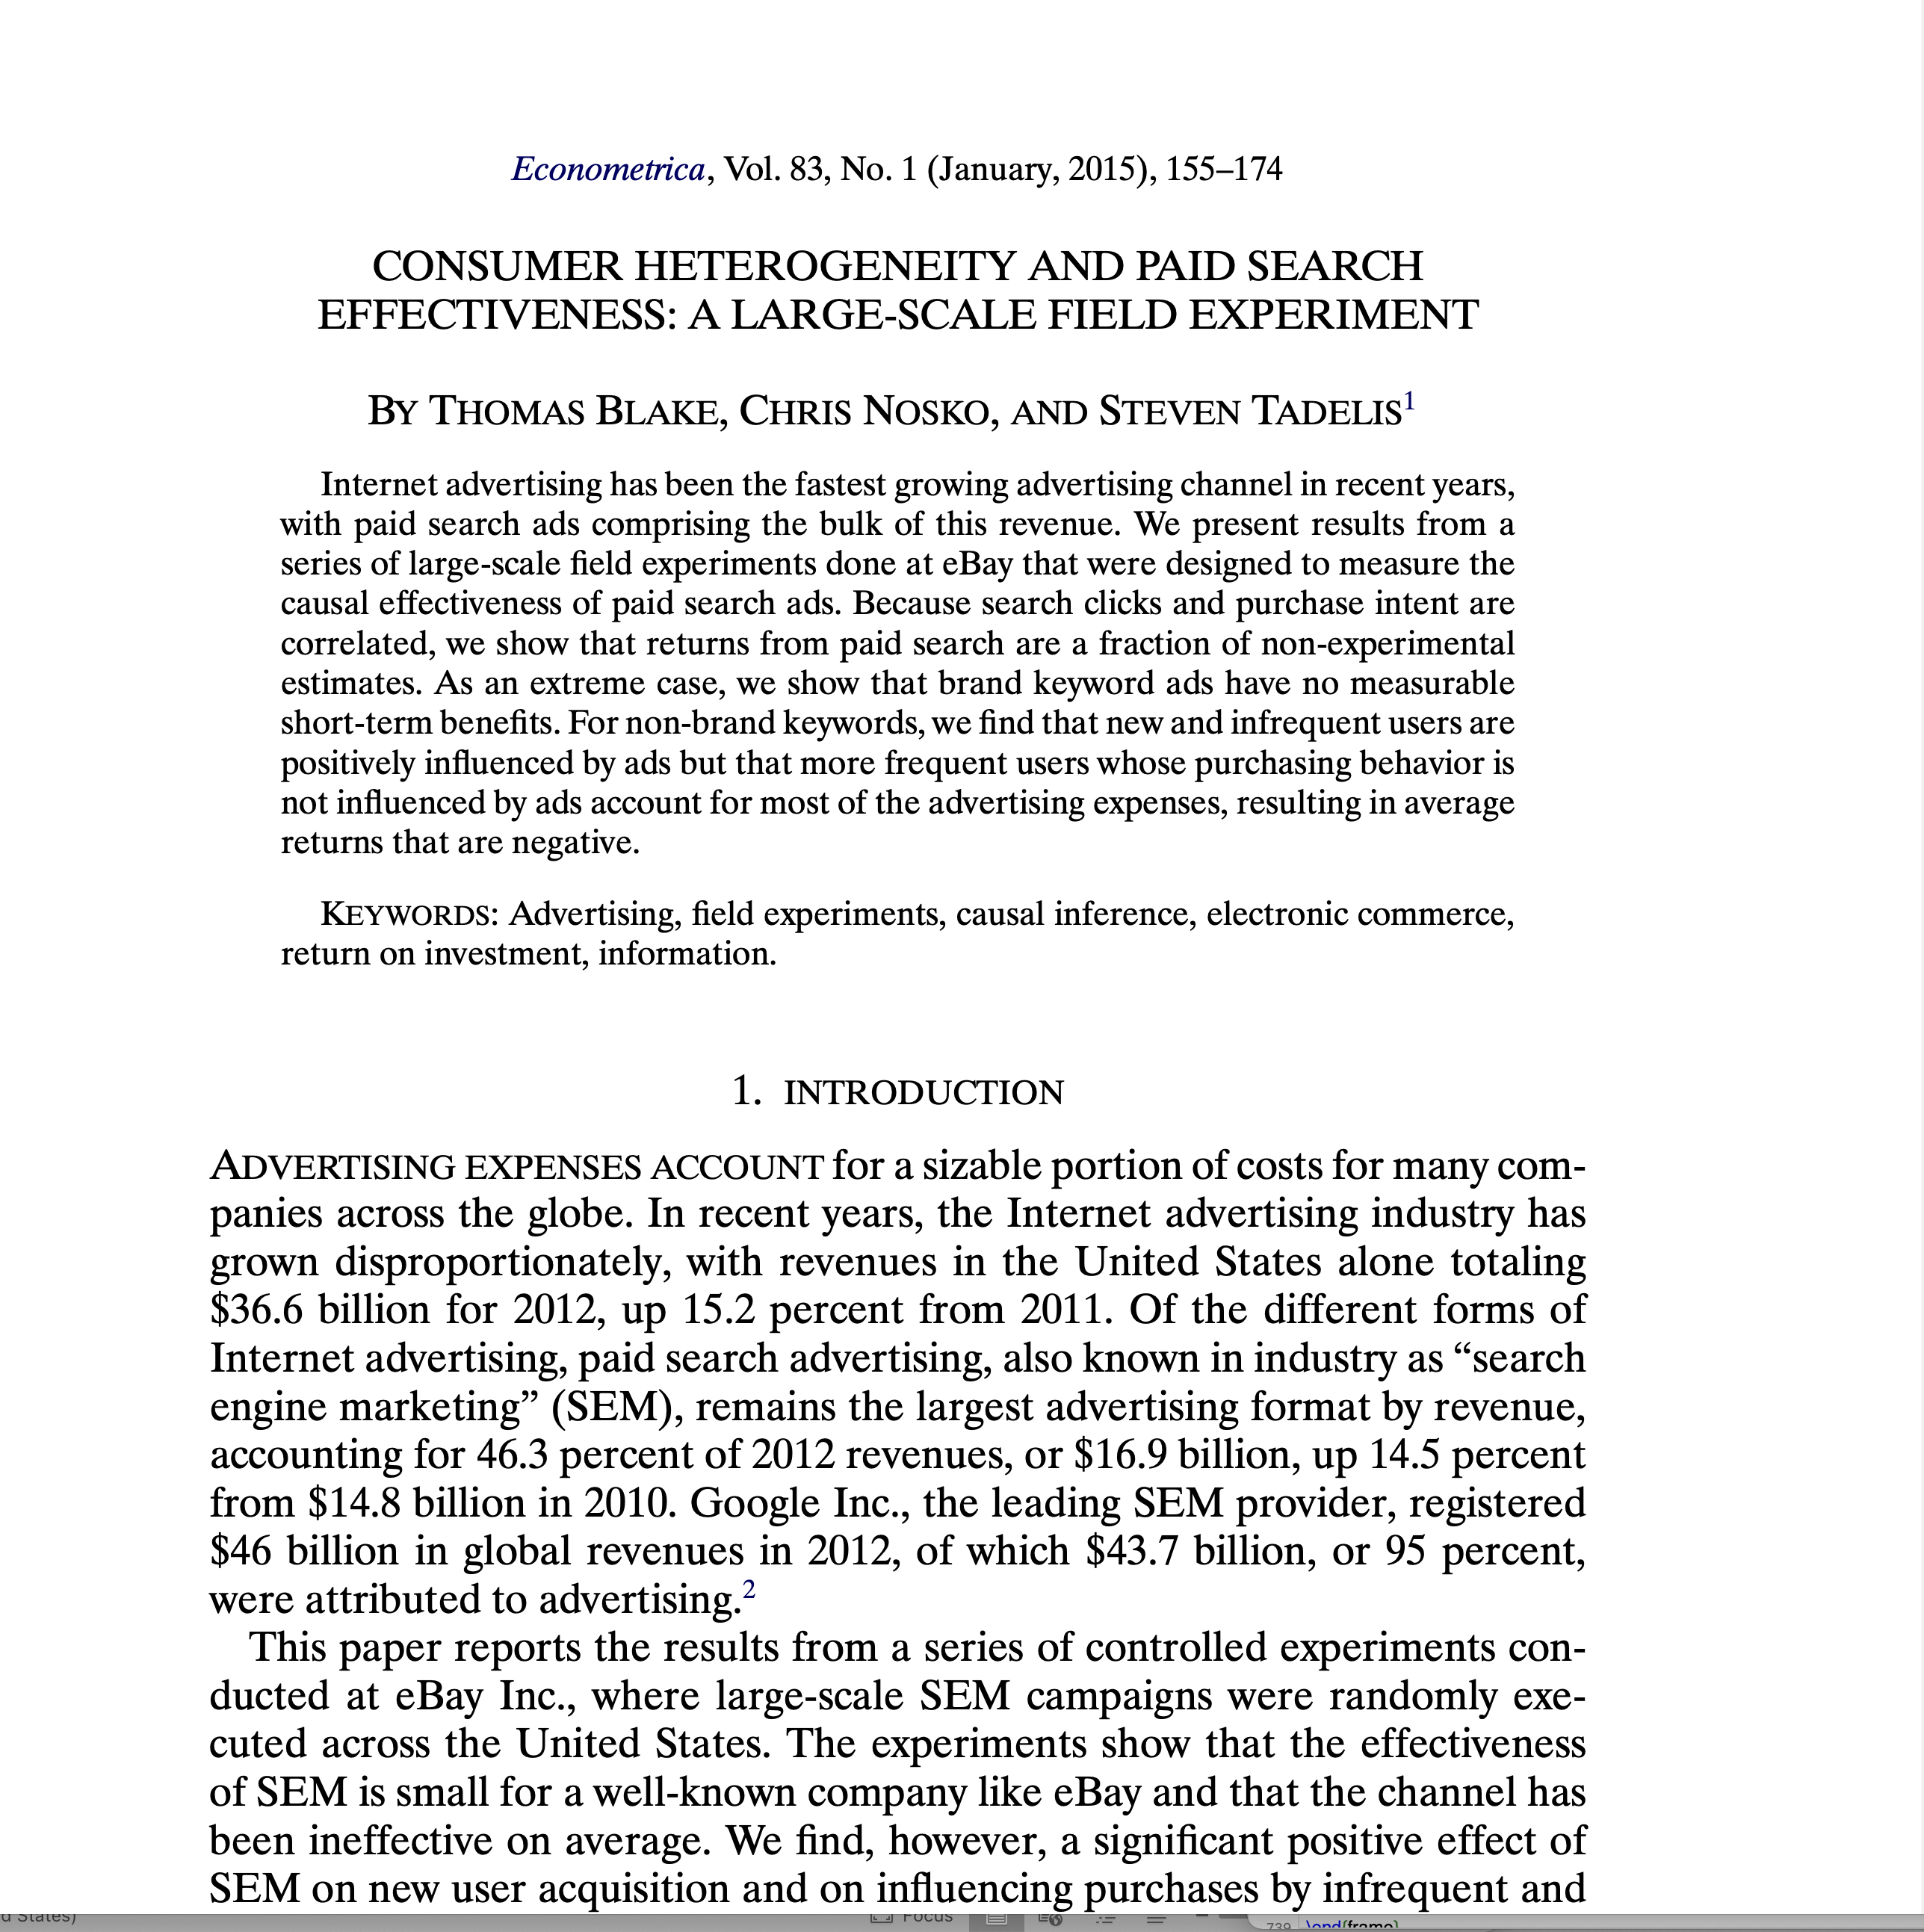
\includegraphics[scale=0.25]{./lecture_includes/econometrica_steve.png}
\end{center}
\end{figure}

\end{frame}

\begin{frame}{Internet advertising facts}

\begin{itemize}
\item In 2012, revenues from Internet advertising was \$36.6 billion and has only grown since
\item Paid search (``search engine marketing'') is the largest format by revenue (46.3\% of 2012 revenues, or \$16.9 billion)
\item Google is leading provider (registered \$46 billion in global revenues in 2012 of which 95\% was attributed to advertising)
\end{itemize}

\end{frame}

\begin{frame}{Selection bias}

\begin{itemize}
\item Treatment was targeted ads at particular people conducting particular types of keyword search
\item Consumers who choose to click on ads are loyal and already informed about products with high likelihood to buy already 
\item Problem is ads are targeting people at the end of their search, so the question is whether they would've found it already (i.e., $E[Y^0|D=1] \neq E[Y^0|D=0]$)
\end{itemize}


\end{frame}



\begin{frame}{Selection bias}

\begin{itemize}
\item Estimated return on investment using OLS  found ROI of over 1600\%
\item Compared this to experimental methods and found ROI of -63\% with a 95\% CI of $[-124\%, -3\%]$, rejecting the hypothesis that the channel yielded short-run positive returns
\item Think back to perfect doctor -- Even without the treatment ($Y^0$), the treated group observationally would've still found a way
\end{itemize}

\end{frame}

\begin{frame}{Natural experiment}

\begin{itemize}
\item Study began with a naturally occurring and somewhat fortuitous  event at eBay
\item eBay halted SEM queries for brand words (i.e., queries that included the term eBay) on Yahoo! and Microsoft but continued to pay for these terms on Google
\item Blake, Nosky and Tadelis (2015) showed almost all of the foregone click traffic and attributed sales were captured by natural search
\item Substitution between paid and unpaid traffic was nearly one to one complete
\end{itemize}

\end{frame}


\begin{frame}

\begin{figure}
\begin{center}
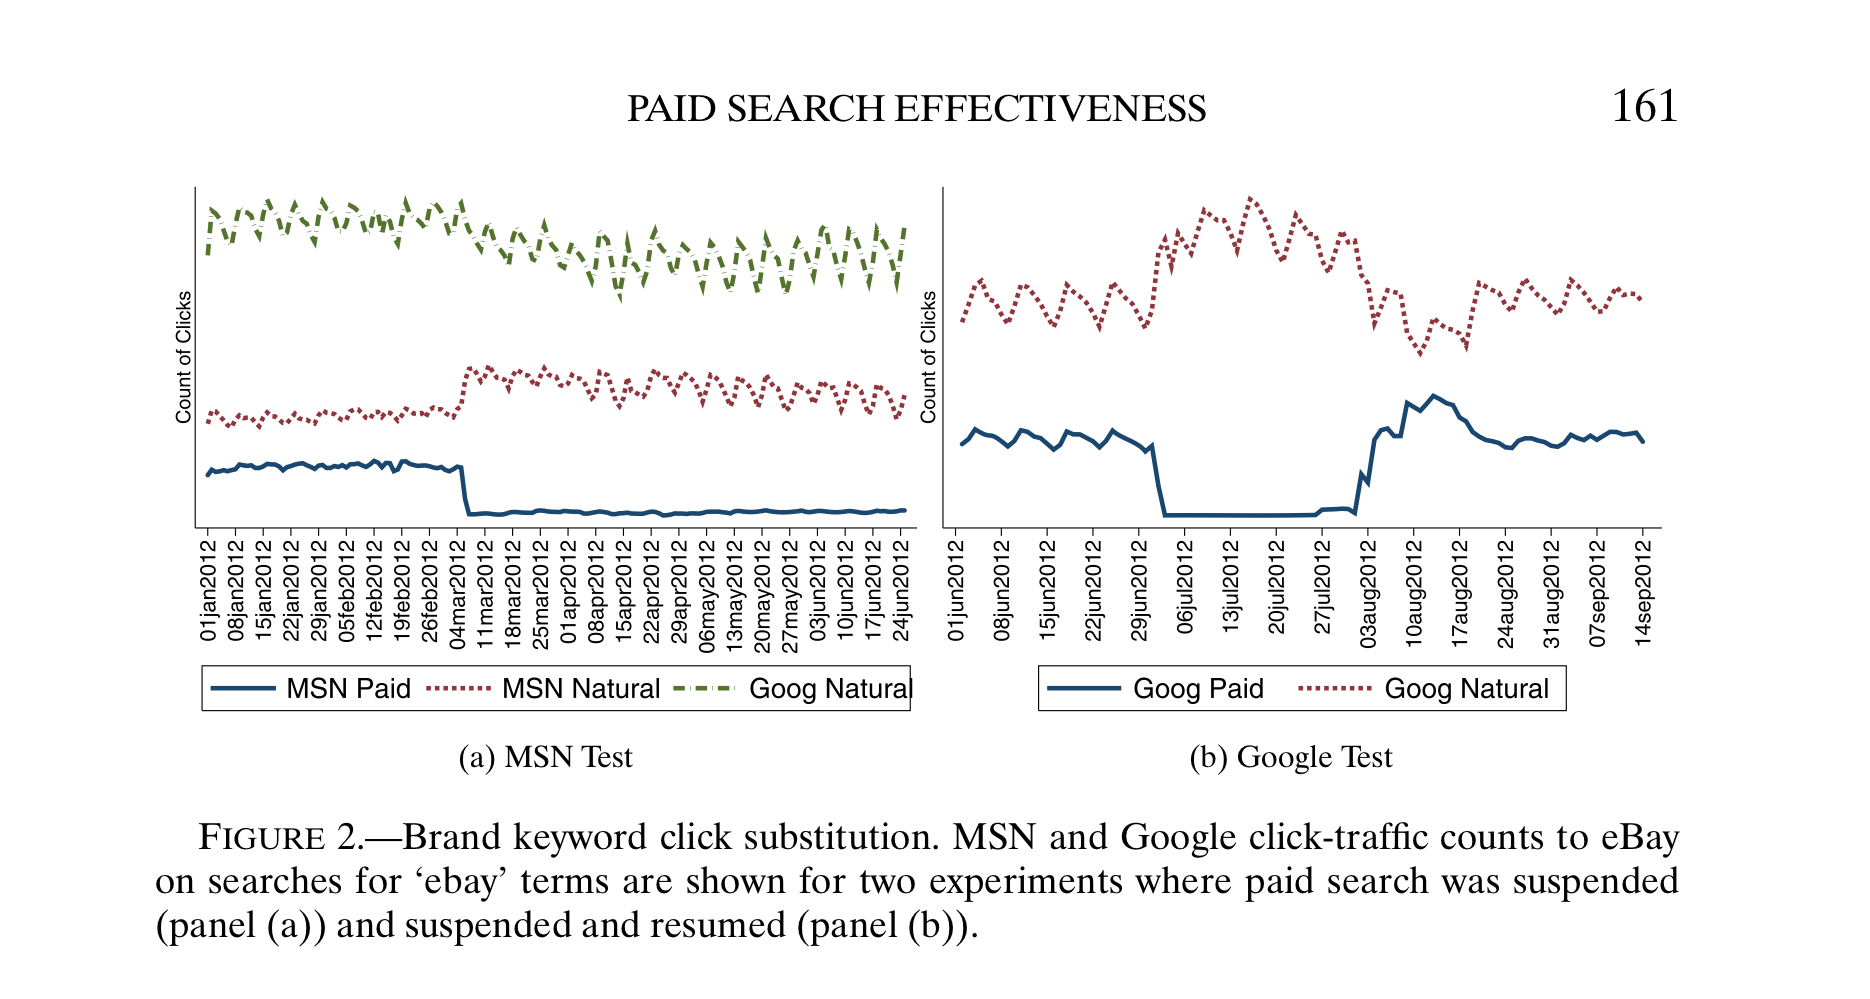
\includegraphics[scale=0.2]{./lecture_includes/tadelis_fig1.png}
\end{center}
\end{figure}

\end{frame}

\begin{frame}{Interpretation of natural experiment}

\begin{quote}
``The evidence strongly supports the intuitive notion that for brand keywords, natural search is close to a perfect substitute for paid search, making brand keyword SEM ineffective for short-term sales.  After all, the users who type the brand keyword in the search query intend to reach the company's website, and most likely will execute on their intent regardless of the appearance of a paid search ad.''
\end{quote}

\end{frame}

\begin{frame}{Selection bias}

Observational data masked causal effect (recall the decomposition of the any non-designed estimation strategy)

\bigskip

\begin{quote}
``Advertising may appear to attract these consumers, when in reality they would have found other channels to visit the company's website.  We overcome this endogeneity challenge with our controlled experiments.''
\end{quote}

\end{frame}




\begin{frame}{RCT}

Natural experiment was valuable, but eBay could run a large scale RCT.

\bigskip


Use this finding of a nearly one-to-one substitution once paid search was dropped to convince eBay to field a large scale RCT discontinuing non-band key words

\bigskip


\end{frame}

\begin{frame}{Design of the experiment}

\begin{itemize}
\item Randomly assigned 30 percent of eBay's US traffic to stop all bidding for all non-brand keywords for 60 days
\item Some random group of users, in other words, were exposed to ads; a control group did not see the ads
\item Used Google's geographic bid feature that can accurately identify geographic market of the user conducting the search
\item Ads were suspended in 30 percent of markets to reduce the scope of the test and minimize the potential cost and impact to the business
\end{itemize}

\end{frame}

\begin{frame}

\begin{figure}
\begin{center}
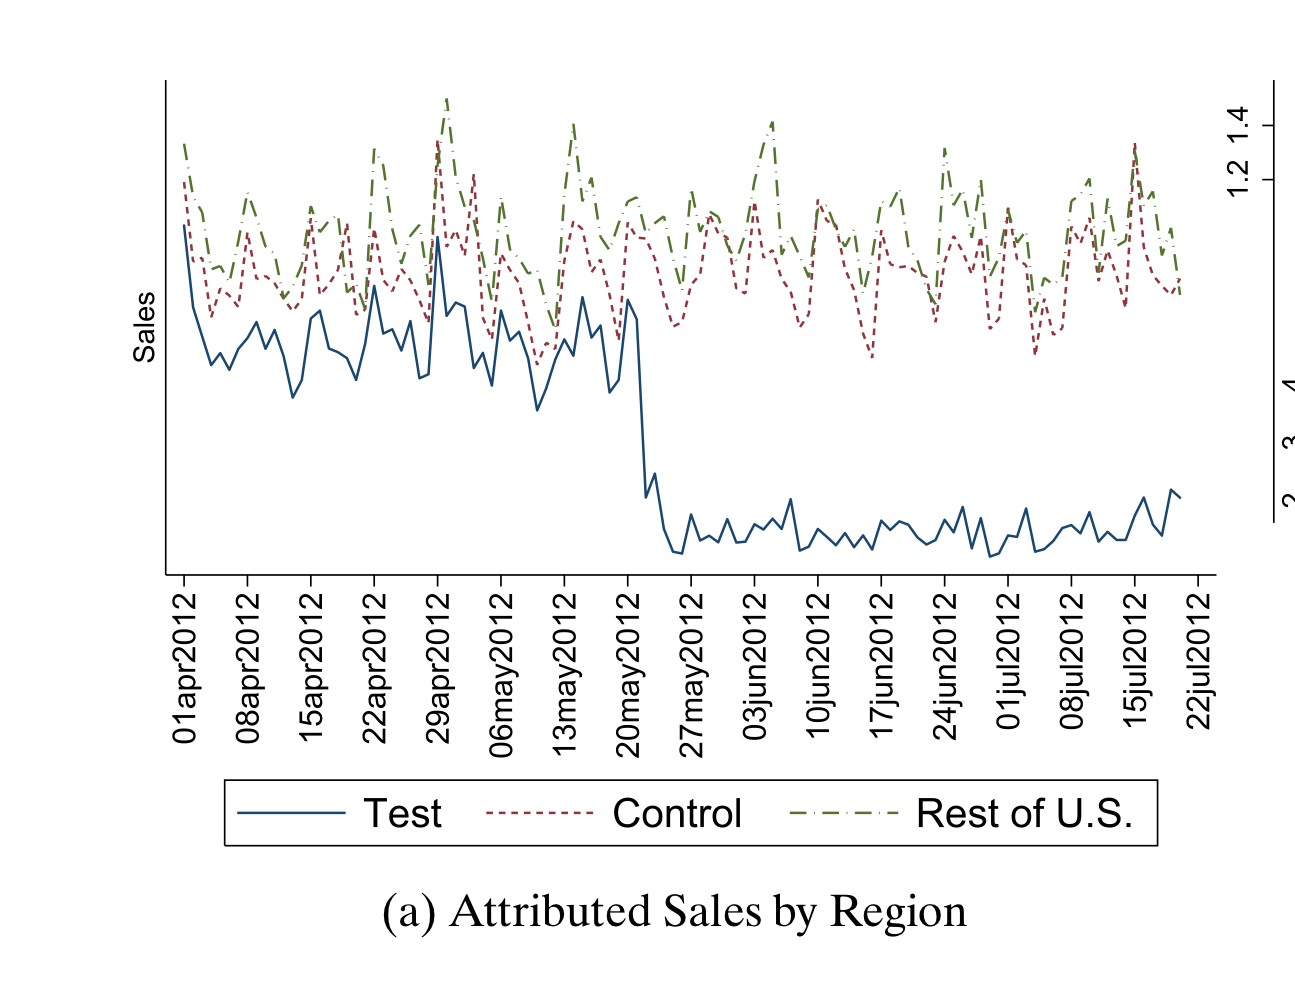
\includegraphics[scale=0.2]{./lecture_includes/tadelis_fig3.png}
\caption{Attributed sales due to clicking on a Google link (treatment group)}
\end{center}
\end{figure}

\end{frame}


\begin{frame}

\begin{figure}
\begin{center}
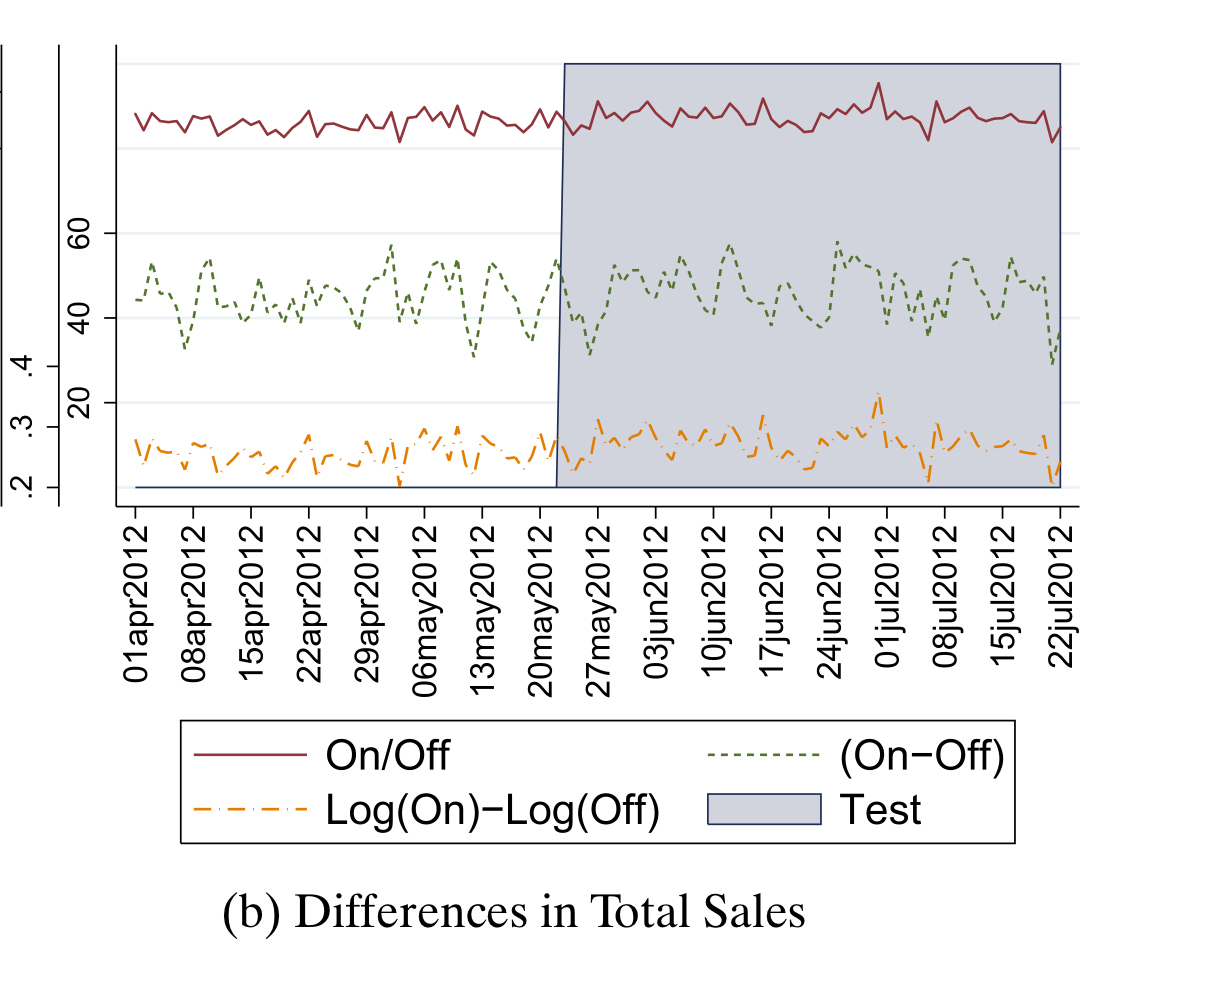
\includegraphics[scale=0.2]{./lecture_includes/tadelis_fig2.png}
\caption{Differences in total sales by market (treatment to control)}
\end{center}
\end{figure}

\end{frame}

\begin{frame}

\begin{figure}
\begin{center}
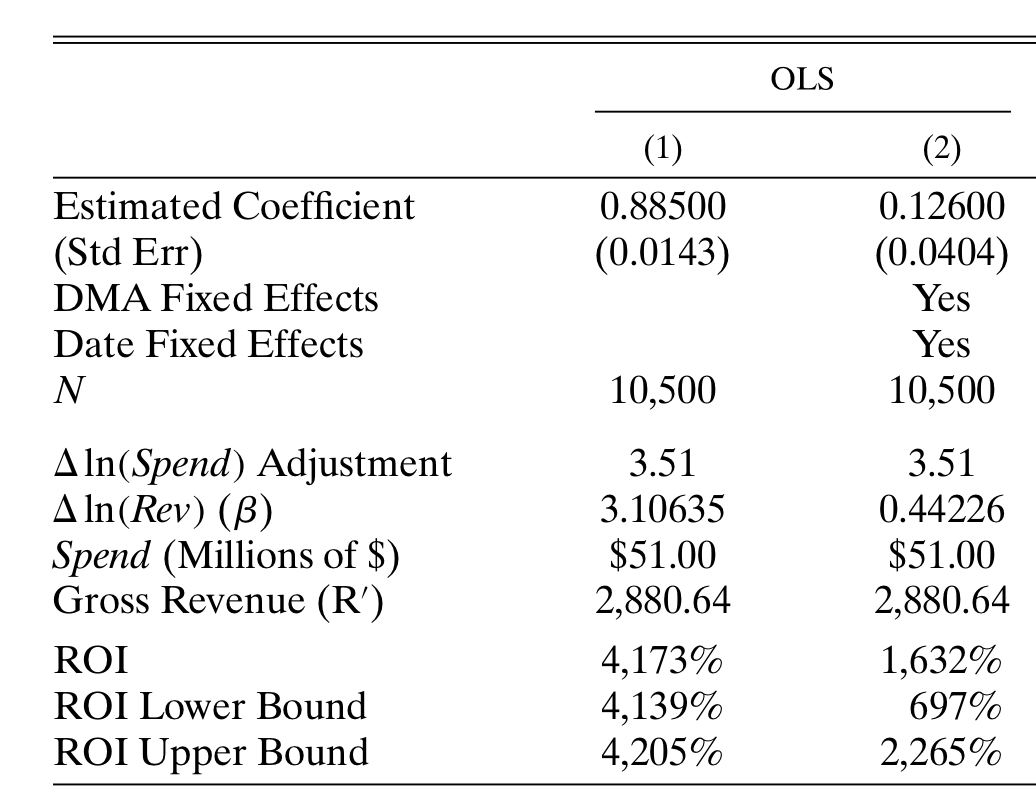
\includegraphics[scale=0.2]{./lecture_includes/tadelis_ols1.png}
\caption{Spending effect on revenue using OLS but not the randomization. Effects are gigantic. }
\end{center}
\end{figure}

\end{frame}

\begin{frame}

\begin{figure}
\begin{center}
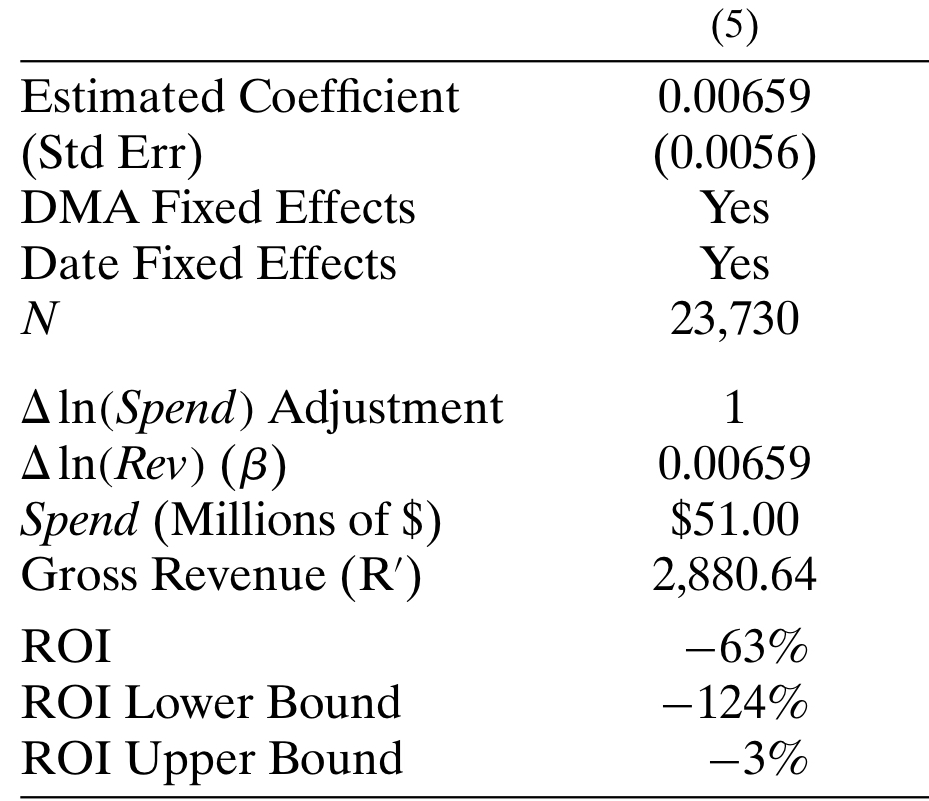
\includegraphics[scale=0.2]{./lecture_includes/tadelis_ols2.png}
\caption{Spending effect on revenue using the randomization. Effects are negative. }
\end{center}
\end{figure}

\end{frame}

\begin{frame}{Heterogenous treatment effects}

\begin{itemize}
\item Recall how the potential outcomes model explicitly models individual treatment effects could be unique and that the perfect doctor showed selection on gains masked treatment effects, perhaps even reversing sign
\item Search advertising in this RCT only worked if the consumer had no idea that the company had the desired product
\item Large firms like eBay with powerful brands will see little benefit from paid search advertising because most consumers already know that they exist, as well as what they have to offer
\end{itemize}

\end{frame}


\begin{frame}

\begin{figure}
\begin{center}
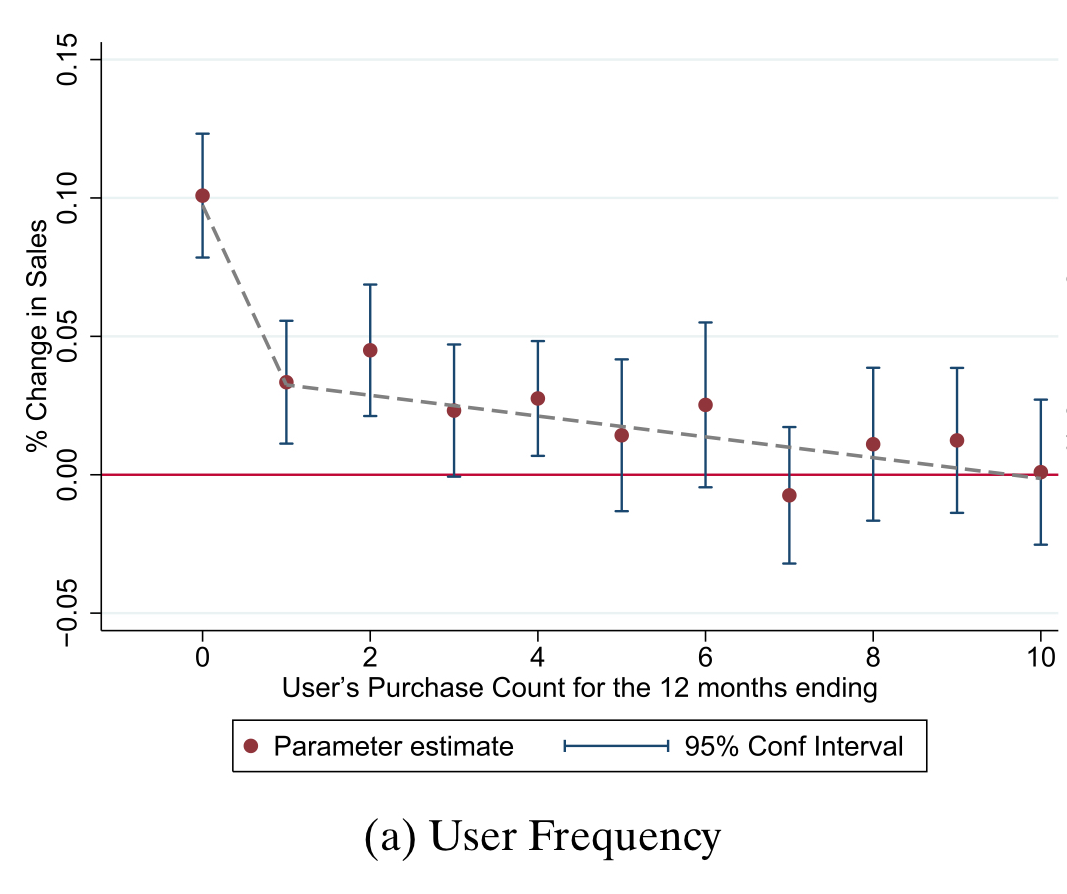
\includegraphics[scale=0.2]{./lecture_includes/tadelis_newuser_fig1.png}
\caption{Effects on new users are positive and large, but not others. }
\end{center}
\end{figure}

\end{frame}

\begin{frame}

\begin{figure}
\begin{center}
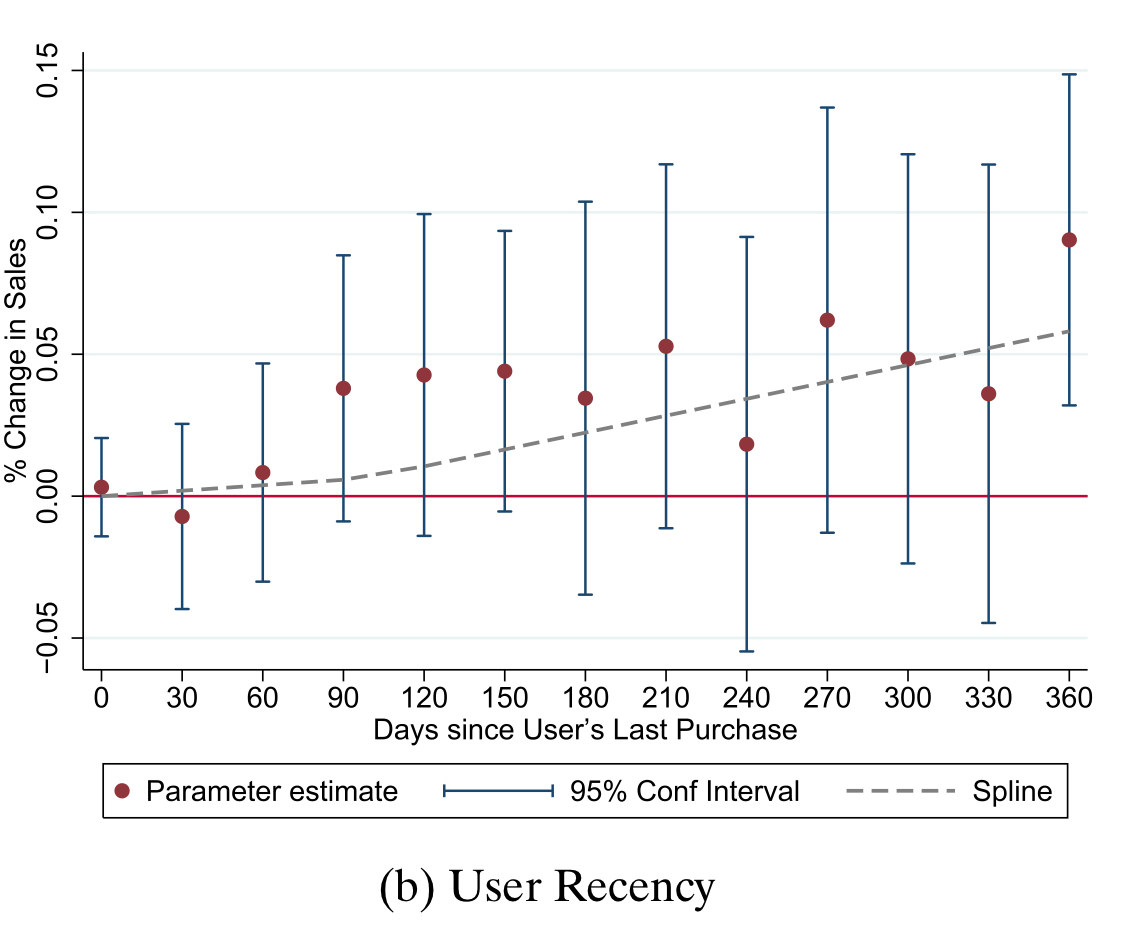
\includegraphics[scale=0.2]{./lecture_includes/tadelis_newuser_fig2.png}
\caption{Effects are largest for ``least active'' customers. }
\end{center}
\end{figure}

\end{frame}


\begin{frame}{Why are causal effects small?}

\begin{itemize}
\item They suggest that the brand query tests found small causal returns because users simply substituted from the paid search clicks to the natural search clicks
\item If that's the case, then it's explicitly a selection bias story $$E[Y^0|D=1] \neq E[Y^0|D=0]$$ where $D$ is being shown the branded advertisement based on search (i.e., they were already going there)
\item They weren't using branded search for information; they were using to \emph{navigate}
\end{itemize}

\end{frame}

\begin{frame}{Self selection based on gains}

\begin{itemize}
\item Potential outcomes is the foundation of the physical experiment because the physical experiment assigns units to treatments \emph{independent} of potential outcomes, $Y^0,Y^1$
\item This is important because outside of the physical experiment, we expect people select those important treatments based on whether, subjectively, they think $Y^1>Y^0$ or $Y^1\leq Y^0$. 
\item Rational actors almost by definition are thought to ``self-select into treatment'' making non-designed comparisons potentially misleading -- sometimes by a little, sometimes by a lot
\end{itemize}

\end{frame}

\section{Tennessee's small class size RCT: STAR}

\begin{frame}[plain]
	\begin{center}
	\textbf{Example 1: Krueger (1999)}
	\end{center}
	
	\begin{itemize}
	\item Krueger (1999) econometrically re-analyzes a randomized experiment to determine the causal effect of class size on student achievement
	\item The project is the Tennessee Student/Teacher Achievement Ratio (STAR) experiment from the 1980s
	\item 11,600 students and their teachers were \emph{randomly} assigned to one of the following three groups:
		\begin{enumerate}
		\item Small class of 13-17 students
		\item Regular class of 22-25 students
		\item Regular class of 22-25 students with a full-time teacher's aide
		\end{enumerate}
	\item After the assignment, the design called for students to remain in the same class type for four years
	\item Randomization occurred within schools
	\end{itemize}
\end{frame}

\begin{frame}[plain,shrink=20]
	\begin{center}
	\textbf{Regression analysis of experiments}
	\end{center}
	
	\begin{itemize}
	\item With randomization one could simply calculate SDO (simple difference in mean outcomes) for the treatment and control group and know that SDO$=$ATE because of independence
	\item Nonetheless, it is often useful to analyze experimental data with regression analysis (see MW section 3.2.2; MHE ch. 2)
	\item Assume that treatment effects are constant -- i.e., $Y^1_i - Y^0_i=\delta$  $\forall i$
	\item Substitute into a rearranged switching equation (Definition 2):
		\begin{eqnarray*}
		Y_i &=& D_iY_i^1 + (1-D_i)Y^0_i \\
		Y_i &=& Y^0_i + (Y^1_i-Y^0_i)D_i \\
		Y_i &=& Y^0_i + \delta D_i  \\
		Y_i &=&E[Y^0_i] + \delta D_i+ Y_i^0 - E[Y_i^0] \\
		Y_i &=& \alpha + \delta D_i + \eta_i
		\end{eqnarray*}where $\eta_i$ is the random part of $Y_i^0$
	\item This is a regression equation that could be used to estimate the causal effect of $D$ on $Y$
	\end{itemize}
\end{frame}

\begin{frame}[plain]
	\begin{center}
	\textbf{Regression analysis of experiments (cont.)}
	\end{center}
	
	\begin{itemize}
	\item The conditional expectation, $E[Y_i|D_i]$, with treatment status switched on and off gives:
		\begin{eqnarray*}
		E[Y_i | D_i=1] &=& \alpha + \delta + E[\eta_i | D_i=1] \\
		E[Y_i | D_i=0] &=& \alpha + E[\eta_i | D_i=0]
		\end{eqnarray*}
	\item Subtracting the latter from the former, we get:
		\begin{eqnarray*}
		 \underbrace{E[Y_i | D_i=1]  - E[Y_i | D_i=0]}_{ \mathclap{\text{SDO}}} &=& \underbrace{\delta}_{ \mathclap{\text{Treatment Effect}}}\\
		 &&+  \underbrace{E[\eta_i | D_i=1] - E[\eta_i | D_i=0]}_{ \mathclap{\text{Selection bias}}}
		\end{eqnarray*}
	\end{itemize}
\end{frame}

\begin{frame}[plain]

\begin{itemize}
	\item We can estimate $SDO$ using least squares but there's other options as well
	\item In the STAR experiment, $D_i$, equalled one if the student was enrolled in a small class and had been \emph{randomly} assigned
	\item Recall that randomization implies that treatment is independent of potential outcomes, and therefore the selection bias vanishes
\end{itemize}
\end{frame}

\begin{frame}[plain]
	\begin{center}
	\textbf{Why Include Control Variables?}
	\end{center}
	
	\begin{itemize}
	\item To evaluate experimental data, one may want to add additional controls in the multivariate regression model.  So, instead of estimating the prior equation, we might estimate:
		\begin{eqnarray*}
		Y_i = \alpha + \delta D_i + X_i'\gamma + \eta_i
		\end{eqnarray*}
	\item There are 2 main reasons for including additional controls in the regression models:
		\begin{enumerate}
		\item Conditional random assignment.  Sometimes randomization is done \emph{conditional} on some observable.  (here that's the school).  We'll discuss ``conditional independence assumption'' when we cover matching.
		\item Additional controls increase precision.  Although control variables $X_i$ are uncorrelated with $D_i$, they may have substantial explanatory power for $Y_i$. Including controls thus reduces variance in the residuals which lowers the standard errors of the regression estimates.
		\end{enumerate}
	\end{itemize}
\end{frame}

\begin{frame}[plain]
	\begin{center}
	\textbf{Regression in Krueger (1999)}
	\end{center}
	
Krueger estimates the following econometric model$$Y_{ics} = \beta_0 + \beta_1 SMALL_{cs} + \beta_2 \text{REG/A}_{cs} + \alpha_s + \varepsilon_{ics}$$\begin{itemize}\item $i$ indexes a student, $c$ indexes a class, and $s$ indexes a school
		\item $Y_{ics}$ is the student's percentile score
		\item $SMALL_{cs}$ is a dummy equalling 1 if she is assigned to a small class.
		\item $REG/A_{cs}$ is a dummy equalling 1 if she was assigned to a regular class with an aide
		\item $\alpha$ is a ``school fixed effect'' which is a vector of school-specific dummy variables.  He conditions on school fixed effects because randomized classroom assignment occurred \emph{within} schools. 
		\end{itemize}
\end{frame}

\begin{frame}[plain]
	\begin{center}
	\textbf{Regression results Kindergarten}
	\end{center}
	
	\begin{figure}
	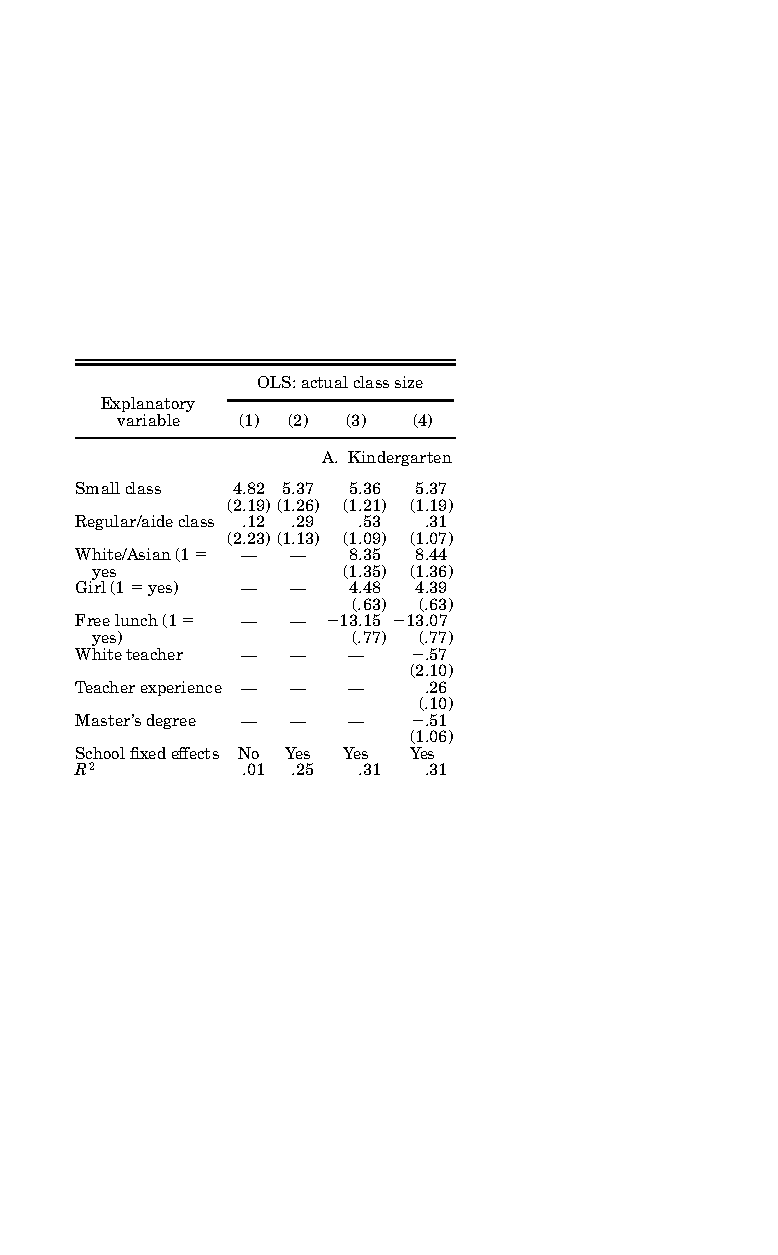
\includegraphics{./lecture_includes/krueger1999_table5a.pdf}
	\end{figure}
\end{frame}


\begin{frame}[plain]
	\begin{center}
	\textbf{Regression results 1st grade}
	\end{center}
	
	\begin{figure}
	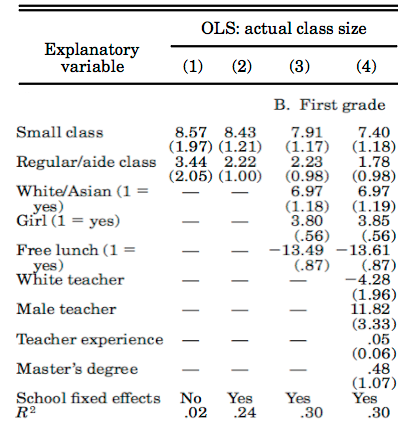
\includegraphics{./lecture_includes/krueger1999_table5b.pdf}
	\end{figure}
\end{frame}

\begin{frame}[plain]
	\begin{center}
	\textbf{Problem 1: Attrition}
	\end{center}
	
A common problem in randomized experiments on humans is \emph{attrition} -- i.e., people leaving the experiment
	\begin{itemize}		
	\item If attrition is random, then attrition affects the treatment and control groups in the same way and our estimates remain unbiased
	\item But in this application, attrition is probably non-random: especially good students from large classes may have enrolled in private schools creating a selection bias problem
	\item Krueger addresses this concern by imputing the test scores (from their earlier test scores) for all children who leave the sample and then re-estimates the model including students with imputed test scores.
	\end{itemize}
\end{frame}

\begin{frame}[plain, shrink=20]
	\begin{center}
	\textbf{Problem 1: Attrition}
	\end{center}
	
	\begin{figure}
	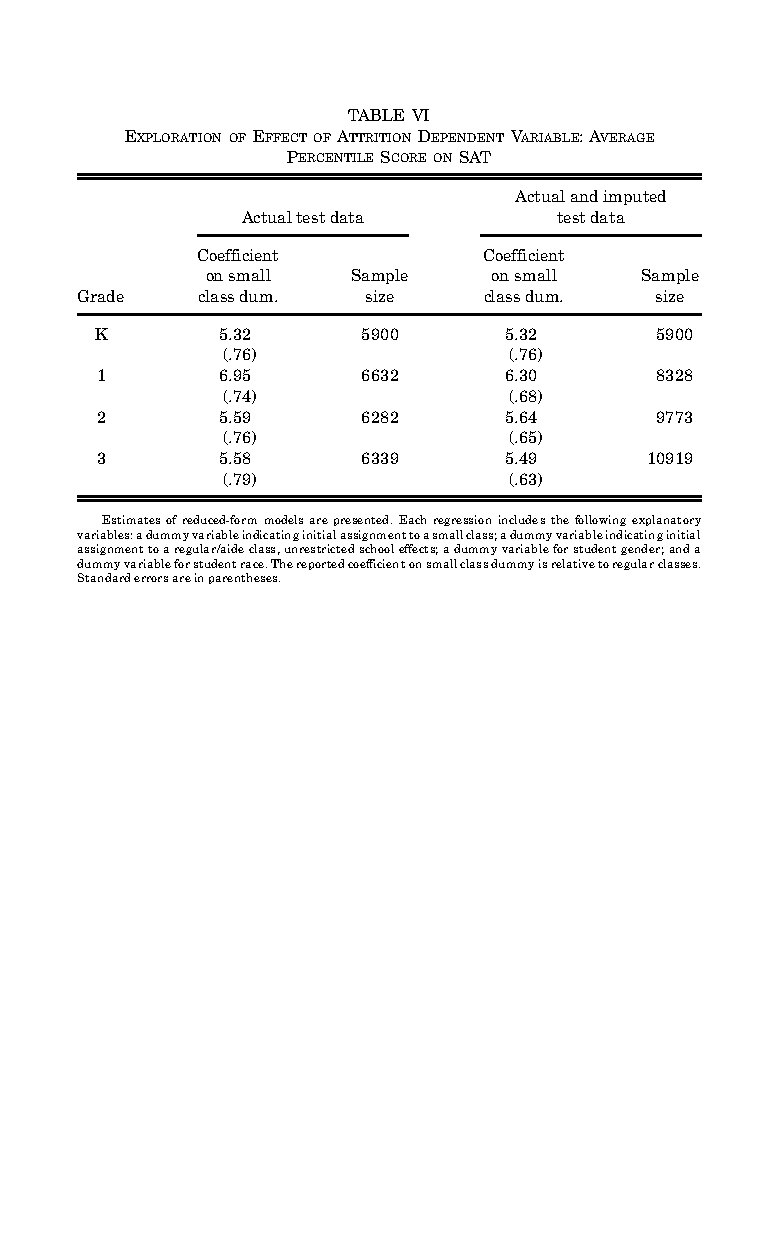
\includegraphics{./lecture_includes/krueger1999_table6.pdf}
	\end{figure}
	
	\begin{itemize}
	\item Non-random attrition hardly biases the results.
	\end{itemize}
\end{frame}

\begin{frame}[plain]
	\begin{center}
	\textbf{Problem 2: Switch Classrooms after Random Assignment}
	\end{center}

``It is virtually impossible to prevent some students from switching between class types over time.'' (Krueger 1999, p. 506)
	\begin{figure}
	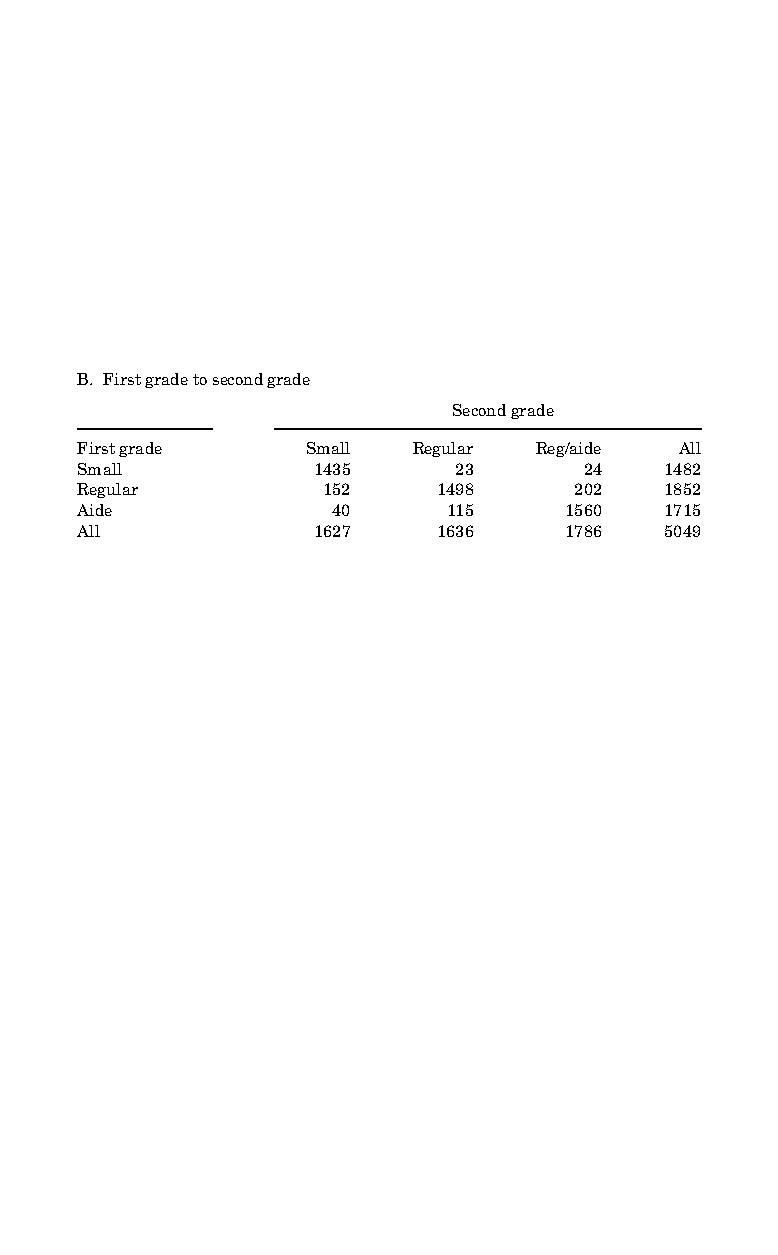
\includegraphics[scale=0.6]{./lecture_includes/krueger1999_table4.pdf}
	\end{figure}

	\begin{itemize}
	\item Interpreting Krueger's``transition matrix'' (above) 
		\begin{itemize}
		\item If students remained in their same class type over time, all the off-diagonal elements would be zero
		\item Interpretation: Of the 1,482 first graders assigned to small classrooms, 1,435 remained in small classes; 23 and 24 switched into regular and regular with aide classes in the second grade
		\end{itemize}
	\item If students with stronger expected academic potential were more likely to move into the small classes, then these transitions would bias a simple comparison of outcomes across class types.
	\end{itemize}
\end{frame}

\begin{frame}[plain]
	\begin{center}
	\textbf{Problem 2: Switch Classrooms after Random Assignment}
	\end{center}

	\begin{itemize}
	\item Subjects moved between treatment and control groups.  How to address this?
	\item A common solution to this problem is to use initial classroom assignment (i.e., small or regular classes) as an \emph{instrument} for actual assignment.  We will discuss instrumental variables later, so I will hold off on that now.
	\item Krueger reports regression results where instead of the student's actual status as the treatment variable, he regresses performance against their \emph{randomly assigned class size}.  This is called the ``reduced form'' model, and we learn more about this when we cover IV.
	\item In Kindergarten, OLS and reduced form are the same because students remained in their initial class for at least one year.
	\item From grade 1 onwards, OLS and reduced form results differ.
	\end{itemize}
\end{frame}

\begin{frame}[plain]
	\begin{center}
	\textbf{Problem 2: Switch Classrooms after Random Assignment}
	\end{center}
	
	\begin{figure}
	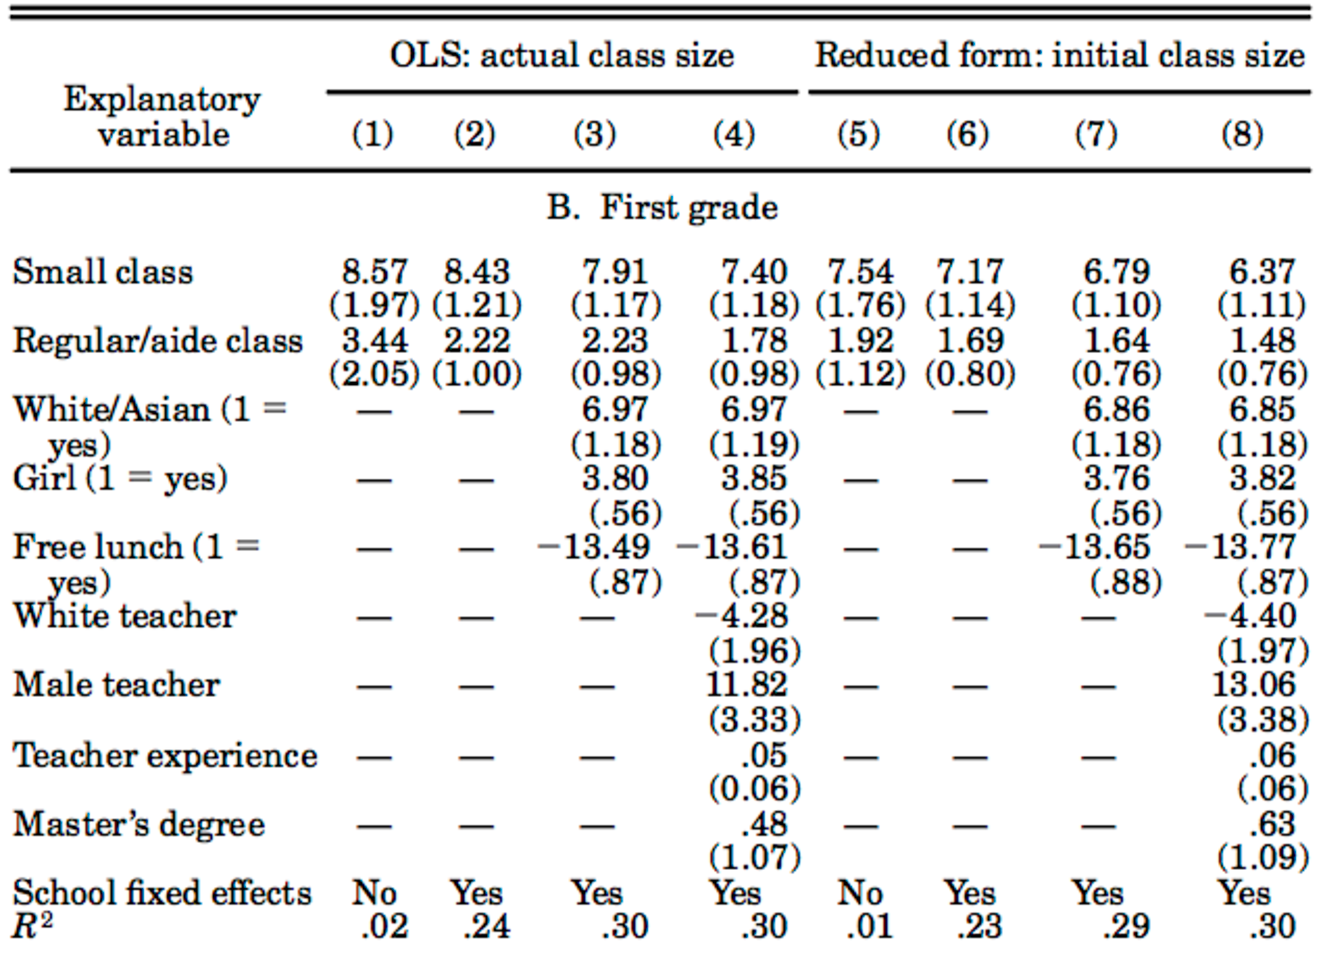
\includegraphics[scale=0.4]{./lecture_includes/krueger1999_table5c.pdf}
	\end{figure}
\end{frame}




\begin{frame}{Comments}

\begin{itemize}
\item Natural experiments are valuable, but they don't always have the same certainty the way an RCT does
\item We use natural experiments when people won't let us run the RCTs we want to run!
\item Findings from natural experiments often push others to run RCTs -- like at eBay
\end{itemize}

\end{frame}


\begin{frame}{Going forward}

\begin{itemize}

\item Now let's move into a set of tools that will help us in two of the areas we cover:  DAGs
\item Matching/regression and instrumental variables both depend critically on knowing something about the data generating process
\item We'll be learning one way to assist you
\end{itemize}

\end{frame}


\begin{frame}{Definition and Identification Come First}

\begin{enumerate}
\item Turn the research question (``what is the causal effect of an advertising campaign on sales?'') into a specific aggregate causal parameter
\item Describe the narrow set of beliefs that make that parameter obtainable with data
\item Build a model that uses the data and the beliefs to estimate the causal parameter?
\end{enumerate}

\bigskip

Most of us skip (1) and many skip (2) and go straight to (3) but hopefully today I'll convince you that that's how errors are introduced, even after one understands that causal inference is not merely correlational

\end{frame}
